% Chapter 3
% Roberto Masocco <robmasocco@gmail.com>
% September 20, 2021

\chapter[Caso di studio: drone autonomo]{Caso di studio: drone autonomo}
\label{chap:Chapter3}
\doublespacing
\fontsize{12}{12}\selectfont
\indent A seguito della discussione portata a termine nei capitoli precedenti circa le nuove soluzioni hardware e software da impiegare per la costruzione di apparati robotici, verrà ora descritto un caso di studio pratico con cui si dimostreranno la validità e l'efficacia di tali strumenti: un drone volante automatico.\\
I task che tale sistema deve svolgere, oltre naturalmente a quelli inerenti il volo in sé, sono specificati nelle regole dell'edizione 2021 del Drone Contest indetto da Leonardo S.p.A. e tenutosi presso la Divisione Velivoli di Leonardo in Corso Francia, Torino. Il prototipo è stato presentato in tale occasione come la proposta del team Asgard Flight Group dell'Università di Roma "Tor Vergata". Il progetto ha coinvolto in tutto cinque tra tesisti e dottorandi afferenti al Dipartimento di Ingegneria Civile e Ingegneria Informatica, i quali sono citati all'inizio di questa Tesi assieme ai loro ruoli e ad un sentito e personale ringraziamento, sotto la supervisione del Prof. Daniele Carnevale. Le regole dell'edizione 2021 del Contest, che costituiscono gli obiettivi operativi del drone, possono essere riassunti come segue:
\begin{itemize}
    \item il drone deve essere in grado di decollare, volare e atterrare autonomamente, orientandosi all'interno di un ambiente indoor di cui è nota a priori la conformazione e la posizione delle piazzole di decollo e atterraggio;
    \item inizialmente il drone deve esplorare l'ambiente, cercando ed individuando dei target mobili costituiti da robot mobili che montano un landmark ArUco;
    \item sono noti solo alcuni dei landmark montati sui robot, dunque quando il drone ne individuasse uno sconosciuto, dovrà scattare ed inviare delle fotografie di esso ad una \emph{Ground Control Station} controllata da un operatore;
    \item sulla base di una stringa di punteggi segnata vicino al landmark del robot, dovrà essere decisa una sequenza di atterraggi sulle varie piazzole;
    \item una volta trasmessa la sequenza al drone, esso dovrà eseguire i vari atterraggi, riconoscendo le piazzole sapendone la posizione nella mappa e rilevando i landmark ArUco dipinti su di esse;
    \item durante tutta la durata del volo deve essere possibile inserire il controllo manuale, per ragioni di sicurezza;
\end{itemize}
Per brevità sono stati tralasciati dei dettagli del regolamento inerenti il solo funzionamento della gara. L'obiettivo finale del Contest è chiaramente la massimizzazione del punteggio ottenuto con gli atterraggi, resa non banale dalla presenza nella mappa di ostacoli, rialzi e zone a bassa visibilità.\\
Nel resto di questo capitolo si descriverà più nel dettaglio il robot, partendo dall'hardware e passando poi al software, da quello di più basso livello fino alle logiche di supervisione e comunicazione con GCS ed operatori.\\
Il prototipo realizzato è ritratto in Figura \ref{fig:drone}, mentre una mappa completa del campo di gara è rappresentata in Figura \ref{fig:map}.

\begin{figure}
    \centering
    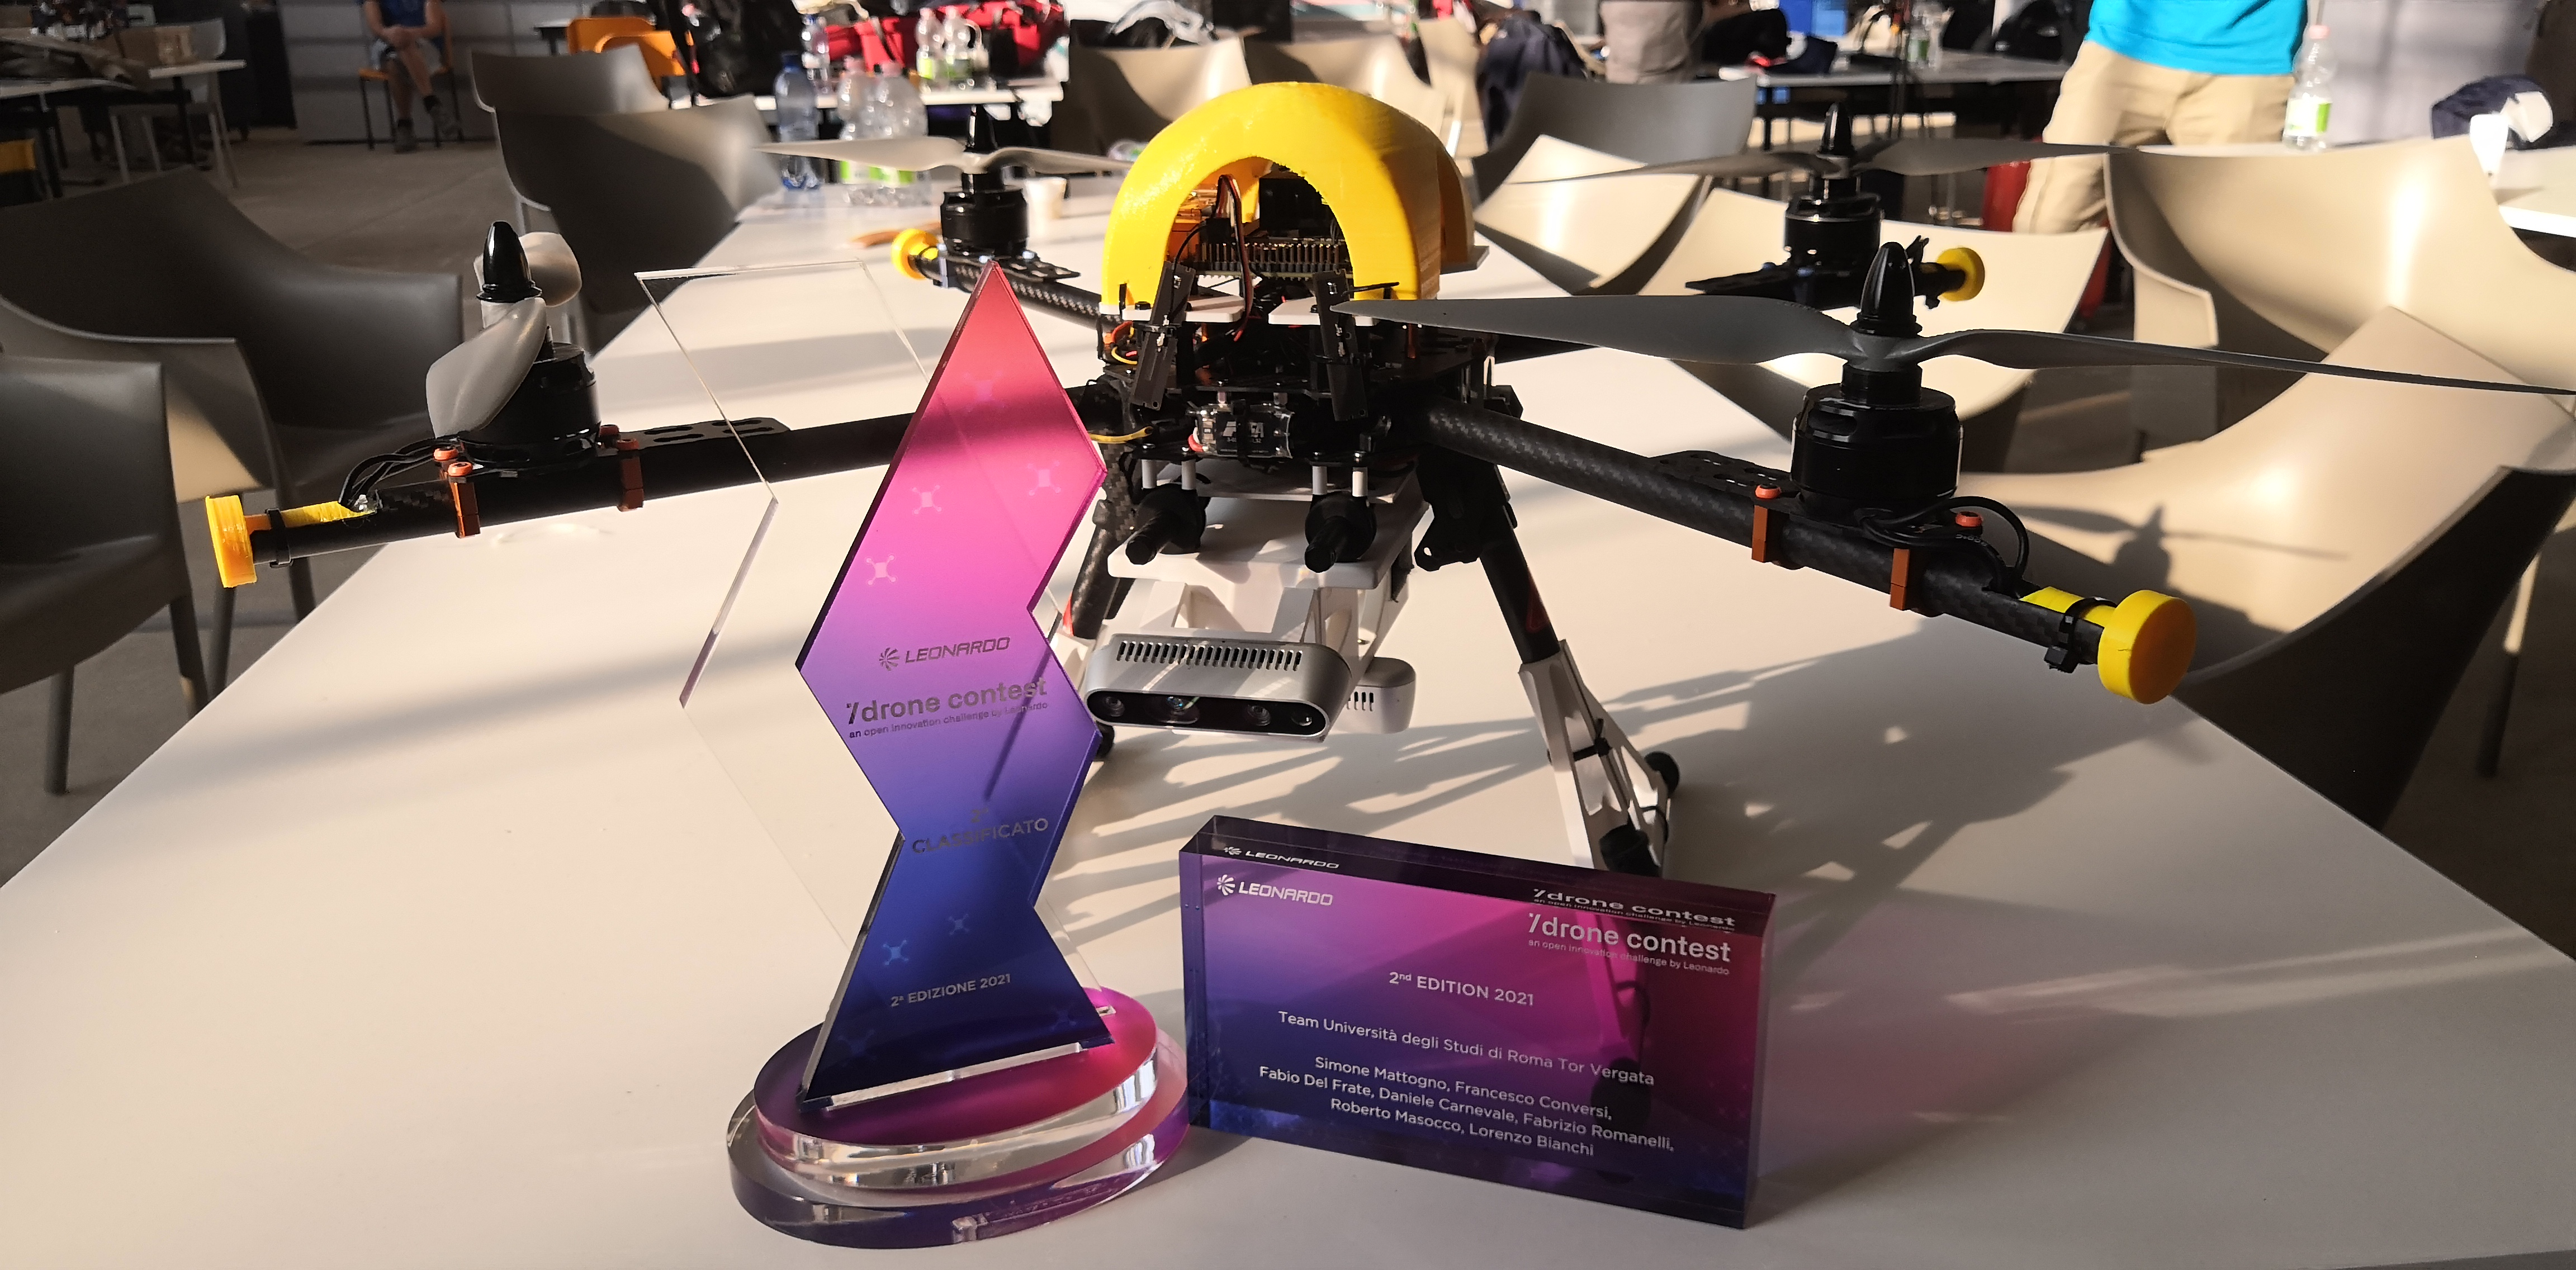
\includegraphics[width=\textwidth]{figs/chapter3/drone.jpg}
    \caption{Prototipo del drone (photo credit: Lorenzo Bianchi).}
    \label{fig:drone}
\end{figure}

\begin{figure}
    \centering
    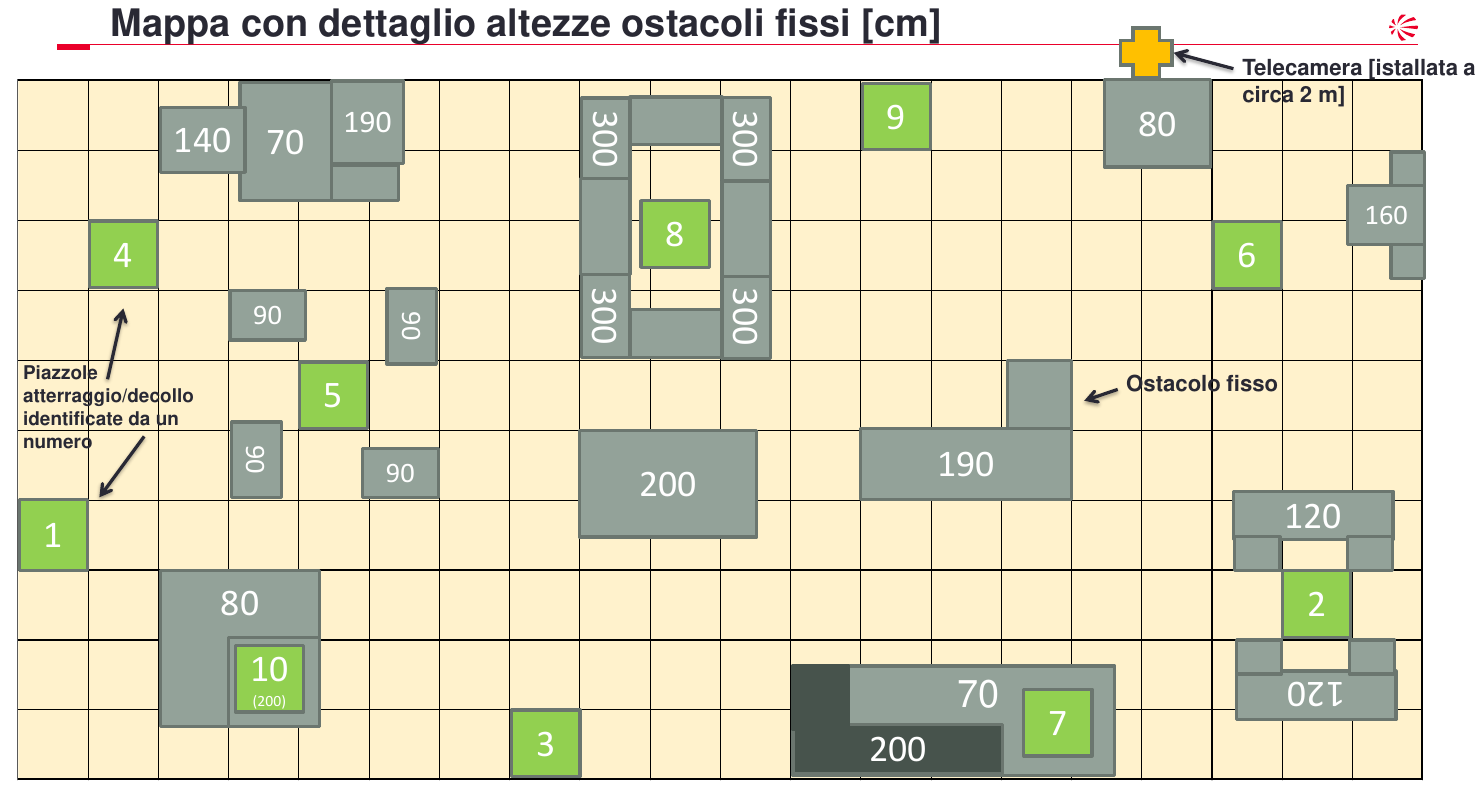
\includegraphics[width=\textwidth]{figs/chapter3/campogara.png}
    \caption{Mappa completa del campo di gara.}
    \label{fig:map}
\end{figure}
\clearpage

\newsection{Hardware}
\newsubsection{Frame e motori}
\indent La primissima decisione progettuale ha riguardato la scelta del \emph{frame}, inteso come struttura portante, su cui montare le varie parti. Nell'economia di un drone volante, in special modo autonomo quindi in grado di stabilizzarsi da solo grazie al feedback di vari sensori di bordo, tale struttura deve essere il più leggera e rigida possibile: il primo requisito riguarda naturalmente le prestazioni, l'autonomia e la controllabilità, mentre il secondo ha risvolti sull'accuratezza delle misure di accelerometri e giroscopi. È infatti comune rilevare durante il volo, mediante uno spettrogramma ricavato dai campioni degli accelerometri, delle vibrazioni dovute a vari fattori. Un esempio è mostrato in Figura \ref{fig:flightspec}, relativo ad una prova di volo automatico in pattugliamento. Prendendola ad esempio, si possono notare dei contributi frequenziali predominanti intorno ai 90 Hz, correlati ad altri precedenti nello spettro e di ampiezza minore: sono le armoniche dei motori. Tali vibrazioni non possono naturalmente essere eliminate, e vanno filtrate e reiezionate dal sistema di controllo e stabilizzazione angolare. Alla fine dello spettrogramma (a circa 6:40) si nota quello che sembra un breve urto, che corrisponde al contatto col suolo in fase di atterraggio, in questo caso preciso e privo di rimbalzo. Eventuali altri contributi significativi, in questo caso assenti, sarebbero indice di problemi meccanici o tarature sbagliate del sistema di controllo.\\
Avendo a che fare con questo genere di prototipo però, è necessario anche uno spazio sufficiente ad ospitare i sistemi elettronici, i sensori e le batterie. Per questo la scelta è ricaduta sul frame Tarot 650, realizzato in carbonio e dotato di una piattaforma centrale sufficientemente ampia da permettere il montaggio dell'elettronica di bordo ricavando due livelli superiori e di un pacco batterie in basso. L'intera struttura è stata pensata avendo cura di spostare il meno possibile lungo la verticale il centro di massa aggiungendo carico al frame: montando la batteria in basso questo tende naturalmente a scendere, imprimendo al sistema un comportamento indesiderato simile a quello di un pendolo composto, caratterizzato da oscillazioni difficili da contrastare. A seguito delle diverse prove e dei vari incidenti di percorso, sono state aggiunte dei pezzi volti a irrobustire i punti più fragili e ridurre ancor di più le vibrazioni. Le ulteriori parti meccaniche necessarie sono state modellate con strumenti CAD e stampate in 3D in PLA e TPU: degli esempi particolarmente rilevanti sono mostrati nelle Figure \ref{fig:batpack}, \ref{fig:frontcam}, \ref{fig:canopy}, \ref{fig:triangle}.\\
Per fornire spinta sono stati montati quattro motori brushless T-Motor U3 da 700 W e 700 rpm/V, dotati di eliche da 12 pollici. Essi sono pilotati dal controllore di volo mediante delle ESC\footnote{Electronic Speed Controller.} F35A BLHeli\_32 digitali a 32 bit con protocollo DShot, configurato per trasmissione a 1200 kpbs. Tale protocollo è particolarmente indicato per la trasmissione di comandi agli attuatori dei droni in quanto garantisce bassissima latenza, robustezza agli errori sui bit, e permette di comunicare direttamente con le ESC per configurarle, consentendo ad esempio di impostare il verso di rotazione dei motori senza dover dissaldarne i cavi per invertire le polarità.

\begin{figure}
    \centering
    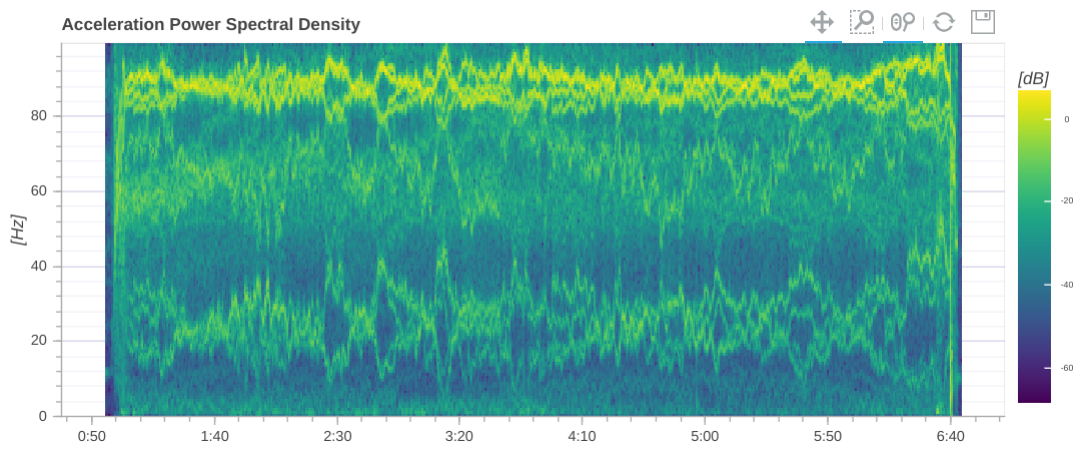
\includegraphics[width=\textwidth]{figs/chapter3/flight_spectro.png}
    \caption{Esempio di spettrogramma ricavato dai dati di un volo automatico.}
    \label{fig:flightspec}
\end{figure}

\begin{figure}
    \centering
    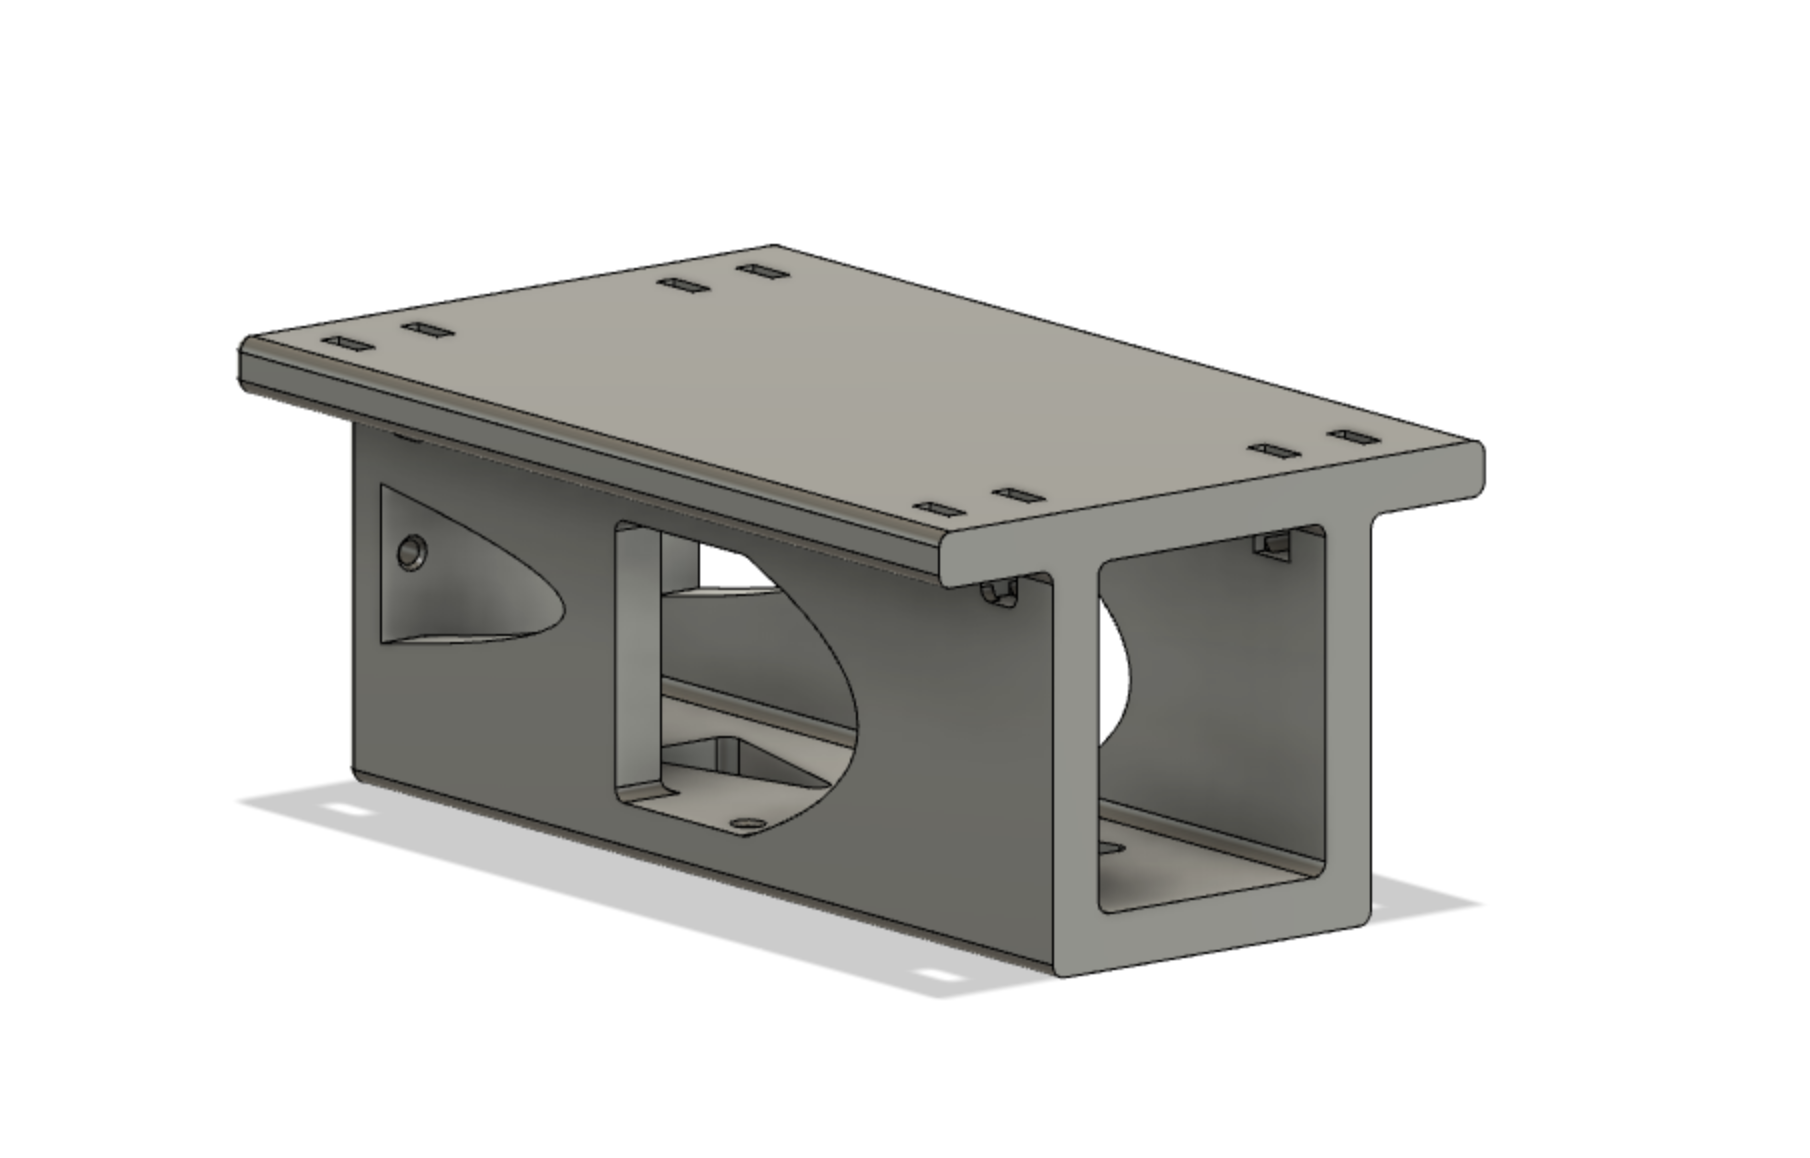
\includegraphics[width=0.9\textwidth]{figs/chapter3/battery-pack.png}
    \caption{Modello CAD del pacco batteria, che funge anche da supporto per la camera inferiore.}
    \label{fig:batpack}
\end{figure}

\begin{figure}
    \centering
    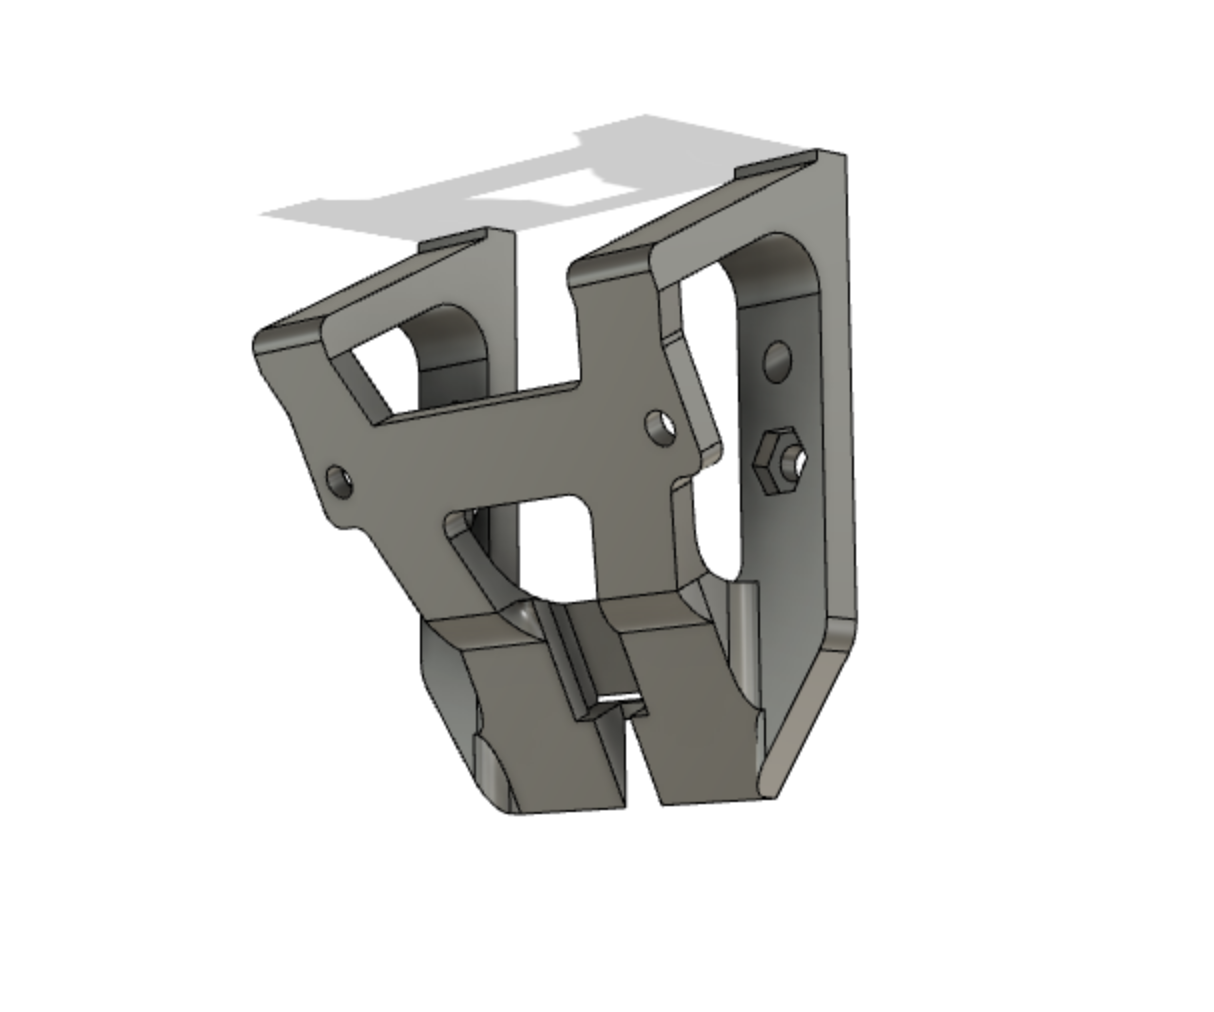
\includegraphics[scale=0.45]{figs/chapter3/camera-holder.png}
    \caption{Modello CAD del supporto della camera frontale, inclinata verso il basso di 26.6°.}
    \label{fig:frontcam}
\end{figure}

\begin{figure}
    \centering
    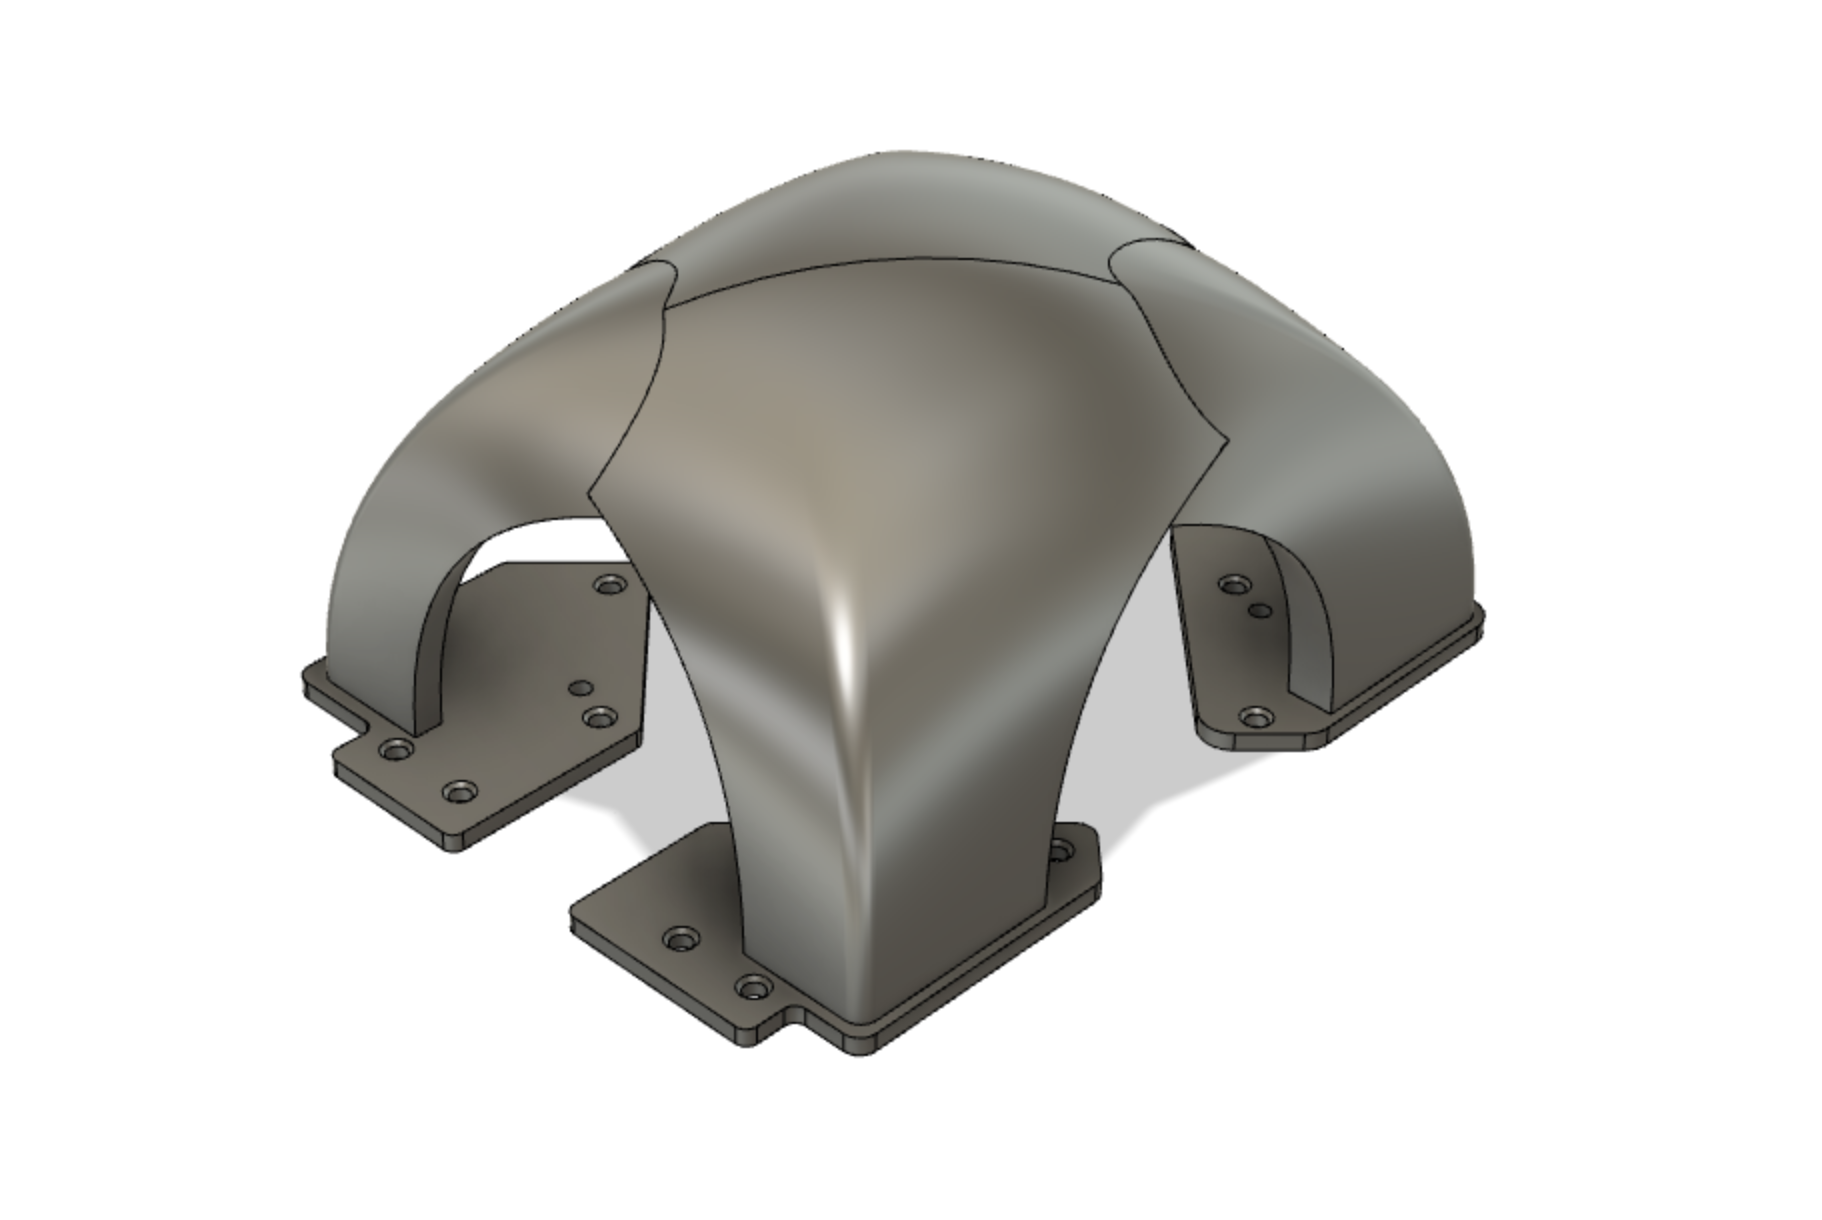
\includegraphics[width=0.9\textwidth]{figs/chapter3/canopy.png}
    \caption{Modello CAD della canopy superiore in TPU, a protezione del computer di bordo.}
    \label{fig:canopy}
\end{figure}

\begin{figure}
    \centering
    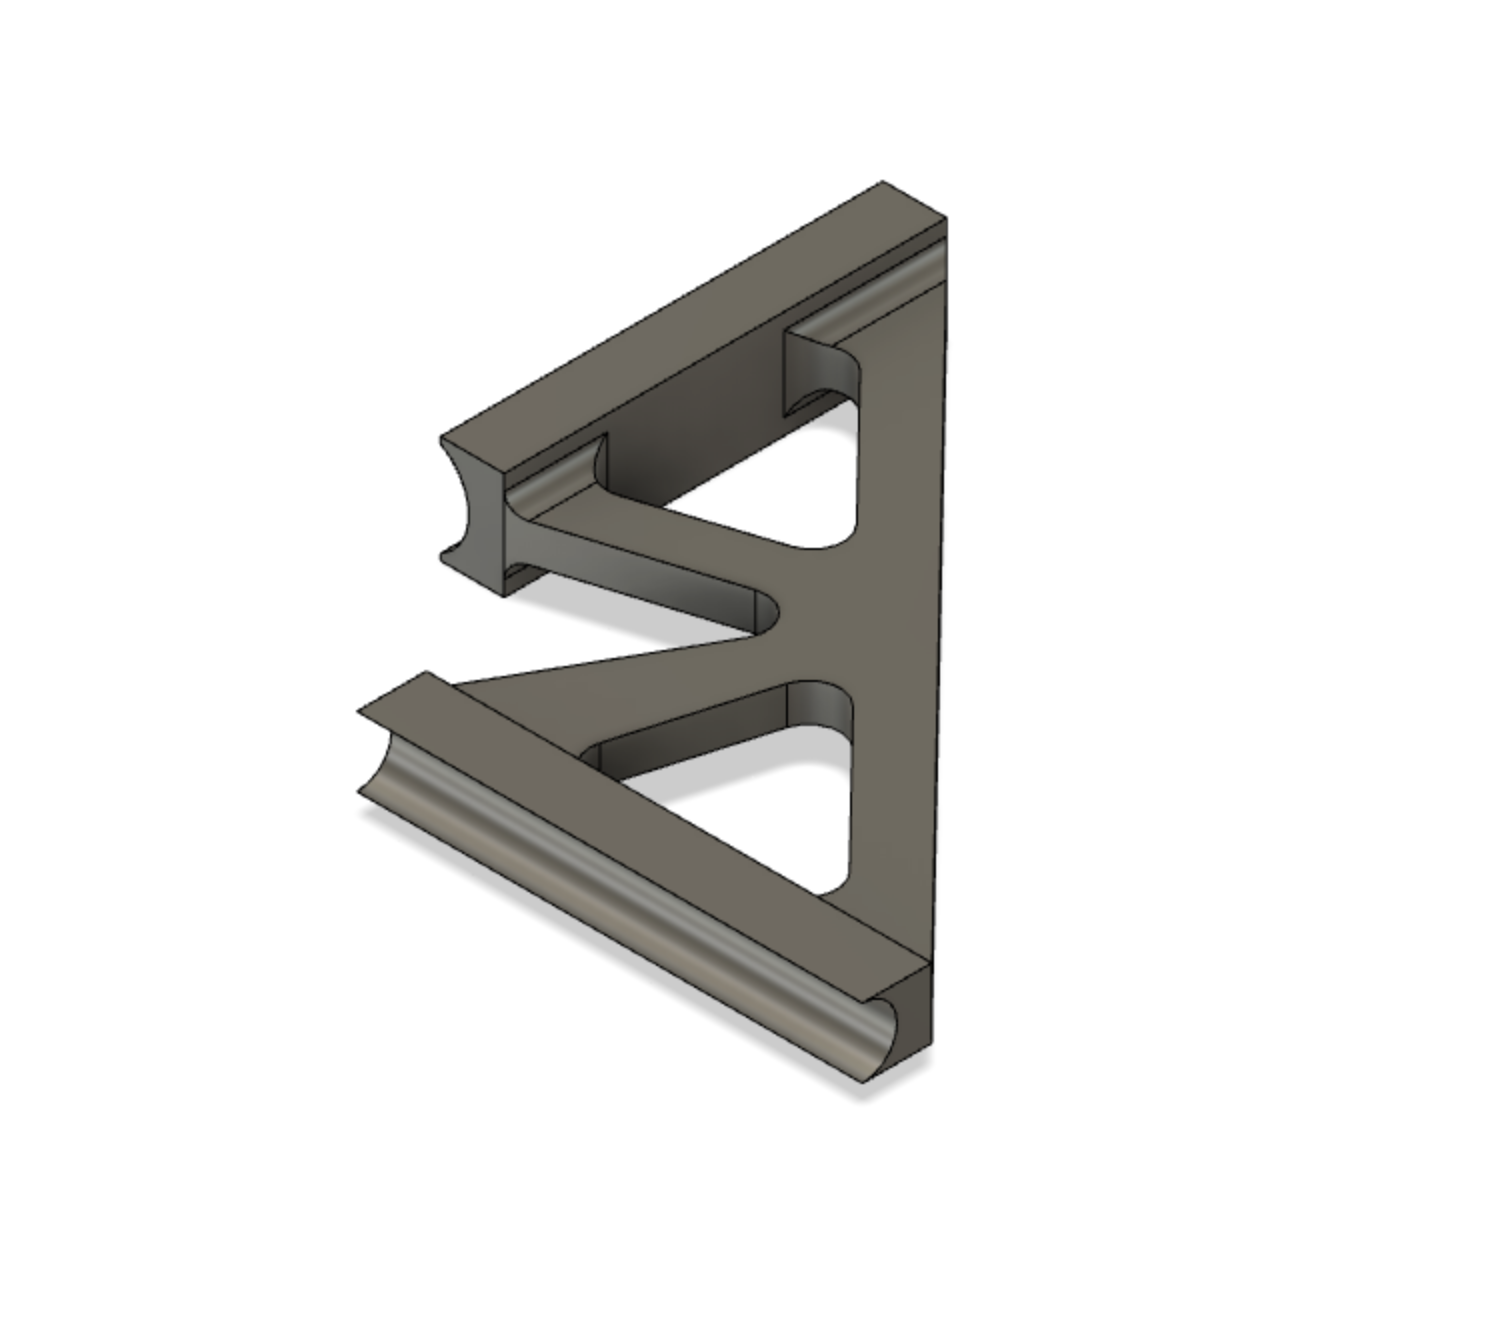
\includegraphics[scale=0.4]{figs/chapter3/triangle.png}
    \caption{Modello CAD del rinforzo triangolare per i carrelli del frame.}
    \label{fig:triangle}
\end{figure}

\newsubsection{Controllore di volo}
\indent La prima parte dell'elettronica di bordo è costituita da un sistema hard real-time\footnote{Con tale locuzione si indica, in genere, un calcolatore elettronico o un controllore numerico per il quale sono specificati una serie di task, ciascuno con delle scadenze temporali precise, e la cui programmazione e realizzazione devono consentire il rispetto tassativo di tali scadenze.} di basso livello, collegato direttamente a sensori e motori, con il compito di localizzarsi in tempo reale e stabilizzare il drone durante le diverse fasi del volo. Per il presente lavoro la scelta è ricaduta sull'Holybro Pixhawk 4, mostrato in Figura \ref{fig:pixhawk}, board compatibile con il firmware open-source PX4 Autopilot\footnote{https://px4.io/}, scritto in C++. Le caratteristiche tecniche principali della board sono riassunte nella Tabella \ref{tab:pix}.\\
\begin{table}
    \centering
    \begin{tabular}{c|c}
        \textbf{CPU} & STM32F765 32 Bit Arm Cortex-M7 \\
        \textbf{I/O Processor} & STM32F100 32 Bit Arm Cortex-M3 \\
        \textbf{Sensori} & IMU\footnote{Una Inertial Measurement Unit è un sistema avionico che implementa il sistema di navigazione inerziale di un aeromobile. È basato su sensori inerziali, come accelerometri e giroscopi, che permettono un monitoraggio della dinamica di un mezzo in movimento.}, magnetometro, barometro, GPS\\
        \textbf{Interfacce} & UART, GPIO, I2C, SPI, CAN, USB
    \end{tabular}
    \caption{Caratteristiche tecniche del controllore di volo Pixhawk 4.}
    \label{tab:pix}
\end{table}
La CPU è dedicata all'esecuzione del firmware PX4 sul Real-Time Operating System NuttX\footnote{https://nuttx.apache.org/}, mentre l'I/O processor all'acquisizione dei dati dai sensori e alla gestione delle interfacce di comunicazione verso ESC o altri componenti. Come da regolamento del Contest, il GPS è stato disattivato e scollegato.\\
Alla board è stata collegata una ricevente radio per aggiungere il controllo manuale con l'ausilio di un radiocomando apposito.\\
La caratteristica saliente di questo controllore è la compatibilità con il progetto PX4. Quest'ultimo, essendo open-source, ha consentito di imparare molto circa il funzionamento e il controllo di un drone, ma anche di intervenire sulla configurazione in modo mirato quando necessario, per eseguire tarature o identificare e risolvere i problemi. I principali servizi offerti da questo firmware, che sono stati ritoccati ed impiegati come parte di questo lavoro per mettere in volo il prototipo secondo le specifiche definite dal Contest, sono i seguenti:
\begin{itemize}
    \item possibilità di controllare il velivolo in posizione, velocità, accelerazione o assetto tramite un computer di bordo esterno;
    \item fusione delle misure acquisite da diversi sensori, sia integrati che esterni ed anche temporalmente sfasati, mediante un filtro di Kalman esteso denominato EKF2\footnote{https://docs.px4.io/master/en/advanced\_config/tuning\_the\_ecl\_ekf.html};
    \item link di comunicazione seriale robusto ad alta velocità verso computer di bordo;
    \vfill
    \item filtri dinamici regolabili per rigettare dalle misure vibrazioni spurie o altri disturbi esterni.
\end{itemize}
L'algoritmo di controllo nonlineare implementato da PX4 è descritto in \cite{px4control}, e una sua schematizzazione è mostrata in Figura \ref{fig:px4controller}, con dettagli nelle Figure \ref{fig:px4angular}, \ref{fig:px4attitude}, \ref{fig:px4velocity}, \ref{fig:px4position}. A ciascun livello, ogni controllore prende in ingresso un riferimento da inseguire e calcola un controllo, da applicare al livello successivo oppure direttamente ai motori tramite opportuno mixing. Ai fini del Contest, tra le modalità disponibili sono state impiegate quelle in posizione e in velocità, a seguito di uno studio accurato del sistema e di una precisa taratura dei suoi vari guadagni e saturazioni.\\
Il sistema di comunicazione con il computer di bordo è invece costituito da un bridge tra due DDS, denominato \emph{microRTPS Bridge}, comprensivo di meccanismi di serializzazione e deserializzazione dei pacchetti in transito sul link seriale. Nello specifico, il firmware integra il DDS basico \emph{uORB}, usato anche per le varie comunicazioni interprocesso nel firmware stesso, mentre l'altro lato della comunicazione è basato su \emph{FastDDS}\footnote{https://www.eprosima.com/index.php/products-all/eprosima-fast-dds} di eProsima. Le due parti della comunicazione seriale sono gestite da due software, uno in esecuzione sul controllore di volo e per questo denominato \emph{Client}, ed uno presente sul computer di bordo e chiamato \emph{Agent}.\\
Tale soluzione assicura una comunicazione affidabile, full-duplex e ad alta velocità tra i due componenti, nonché la semplice integrazione con altri middleware quali ad esempio ROS 2. Anche questo progetto è open-source, ed è stato modificato in svariati punti durante questo lavoro al fine di produrre una versione migliore di quella ufficiale, nella quale sono state rilevate gravi mancanze nella gestione di eventuali pacchetti malformati, che potevano portare casualmente al crash del programma. Una schematizzazione dell'architettura di comunicazione è mostrata in Figura \ref{fig:rtpsbridge}.

\begin{figure}
    \centering
    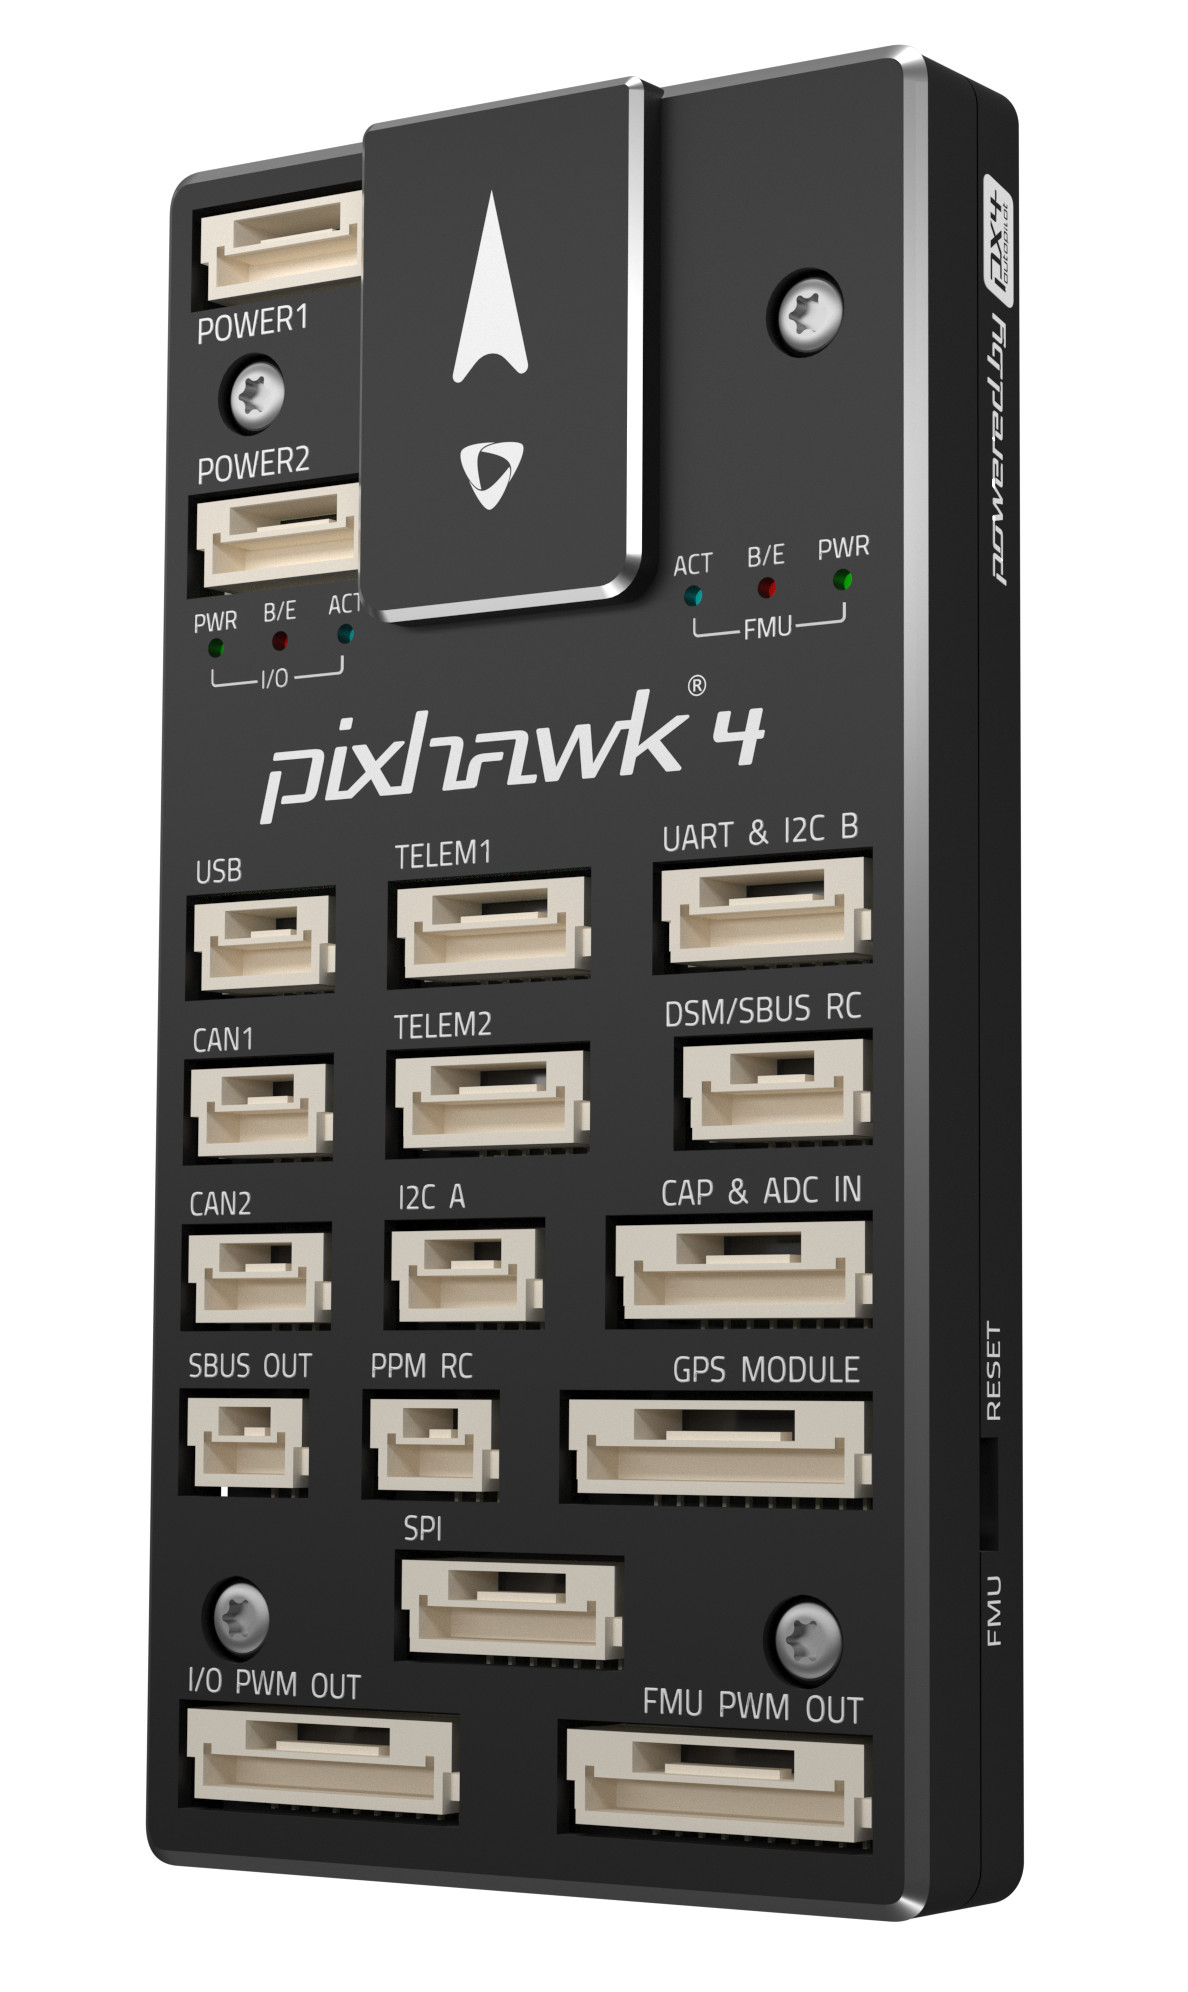
\includegraphics[scale=0.1]{figs/chapter3/pixhawk4.jpg}
    \caption{Controllore di volo Pixhawk 4.}
    \label{fig:pixhawk}
\end{figure}

\begin{figure}
    \centering
    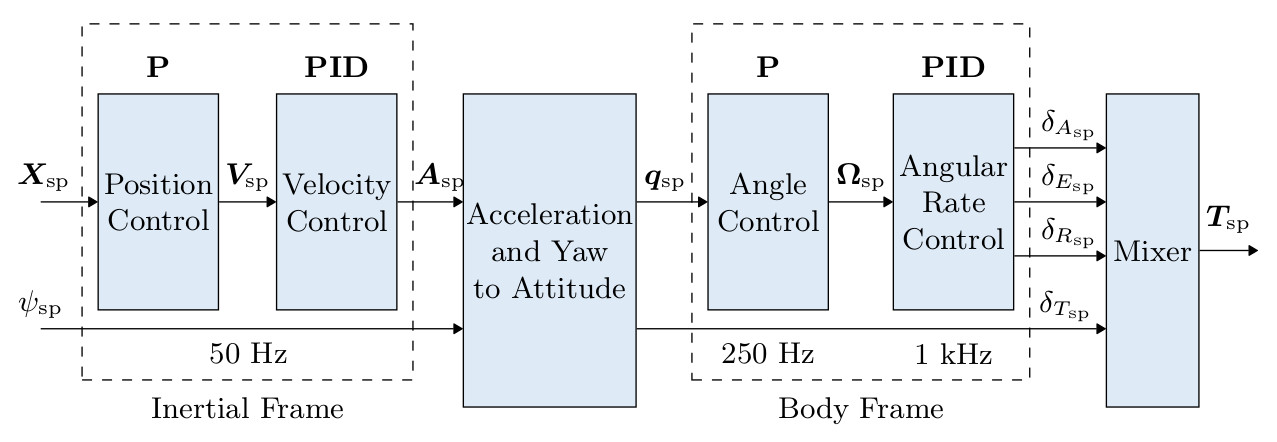
\includegraphics[width=0.9\textwidth]{figs/chapter3/px4-controller.jpg}
    \caption{Schema del controllore di volo multilivello implementato da PX4, con i diversi tempi di campionamento dei vari sottosistemi.}
    \label{fig:px4controller}
\end{figure}

\begin{figure}
    \centering
    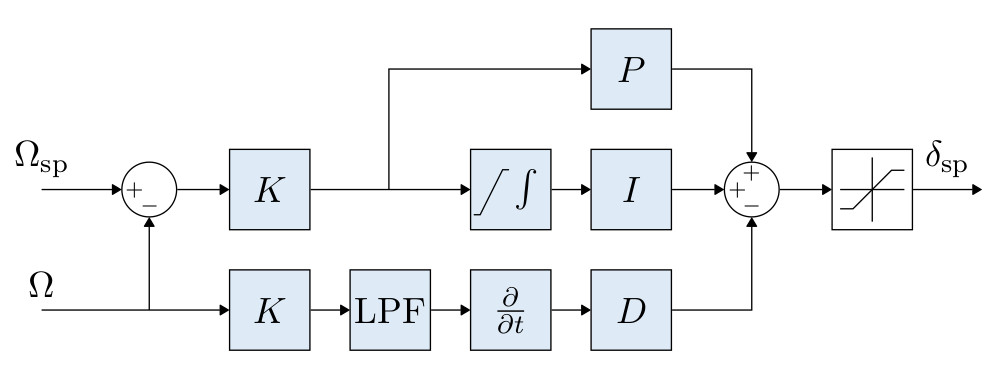
\includegraphics[width=0.9\textwidth]{figs/chapter3/px4-angularcont.jpg}
    \caption{Dettaglio del controllore PID con filtri per la stabilizzazione angolare.}
    \label{fig:px4angular}
\end{figure}

\begin{figure}
    \centering
    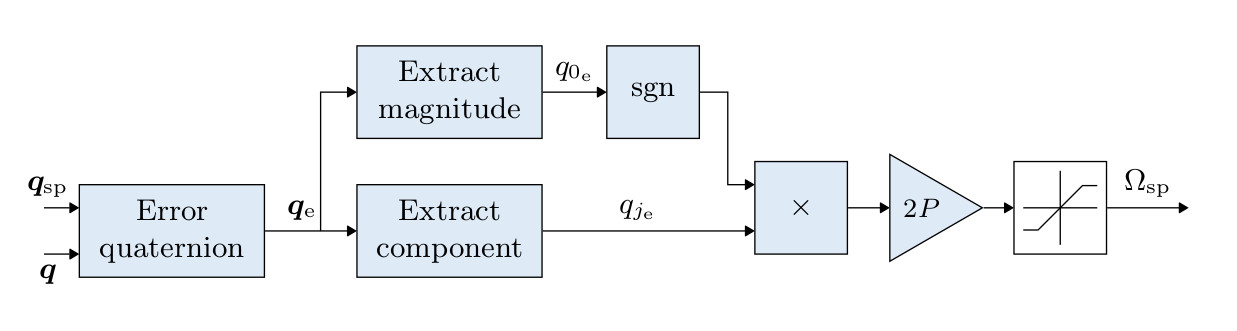
\includegraphics[width=0.9\textwidth]{figs/chapter3/px4-attitude.jpg}
    \caption{Dettaglio del controllore di PX4 per la regolazione dell'assetto basato, sui quaternioni d'orientamento.}
    \label{fig:px4attitude}
\end{figure}

\begin{figure}
    \centering
    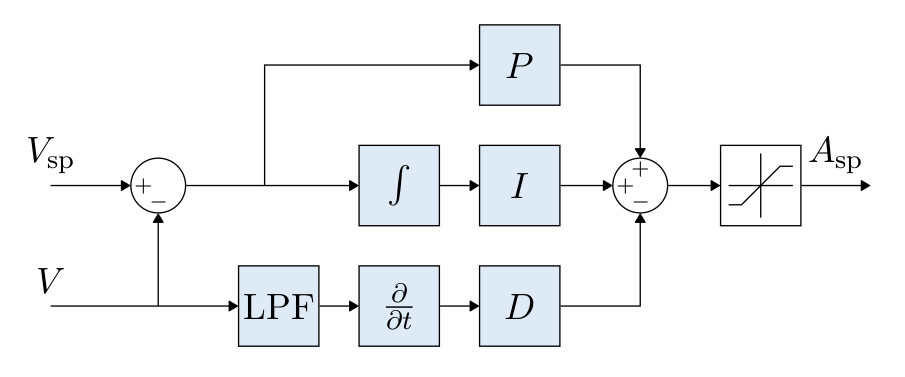
\includegraphics[width=0.9\textwidth]{figs/chapter3/px4-velocity.jpg}
    \caption{Dettaglio del controllore PID con filtri per la regolazione della velocità lineare.}
    \label{fig:px4velocity}
\end{figure}

\begin{figure}
    \centering
    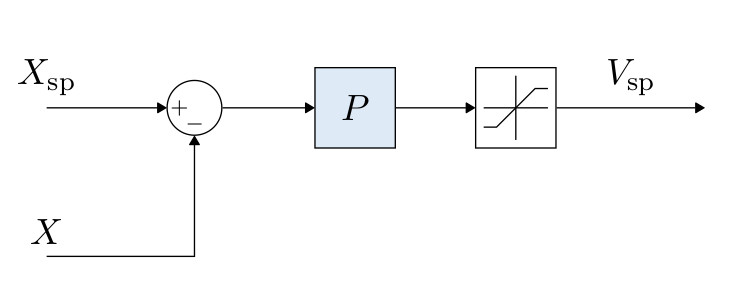
\includegraphics[width=0.7\textwidth]{figs/chapter3/px4-position.jpg}
    \caption{Dettaglio del controllore proporzionale per l'inseguimento della posizione.}
    \label{fig:px4position}
\end{figure}

\begin{figure}
    \centering
    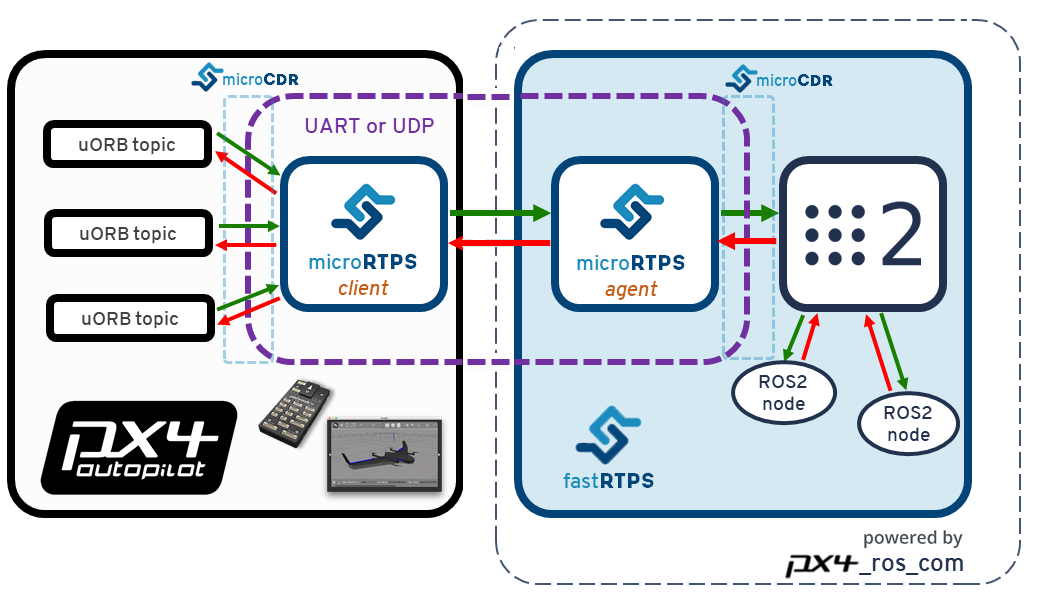
\includegraphics[width=0.9\textwidth]{figs/chapter3/rtps-bridge.png}
    \caption{Architettura del link di comunicazione microRTPS Bridge.}
    \label{fig:rtpsbridge}
\end{figure}

\newsubsection{Fotocamere}
\indent Al fine di riconoscere i target montati sui robot mobili a terra, nonché di localizzarsi nell'ambiente, si sono rese necessarie due fotocamere, montate rispettivamente di fronte e verso il basso. La scelta è ricaduta sulle Intel RealSense D435i (Figura \ref{fig:d435i}), dotate di interfaccia USB 3.1 e vari sensori, dei quali sono stati usati le camere RGB e ad infrarossi per ricavare una mappa di profondità. L'integrazione col resto del software è stata possibile mediante dei driver open-source resi disponibili da Intel.

\begin{figure}
    \centering
    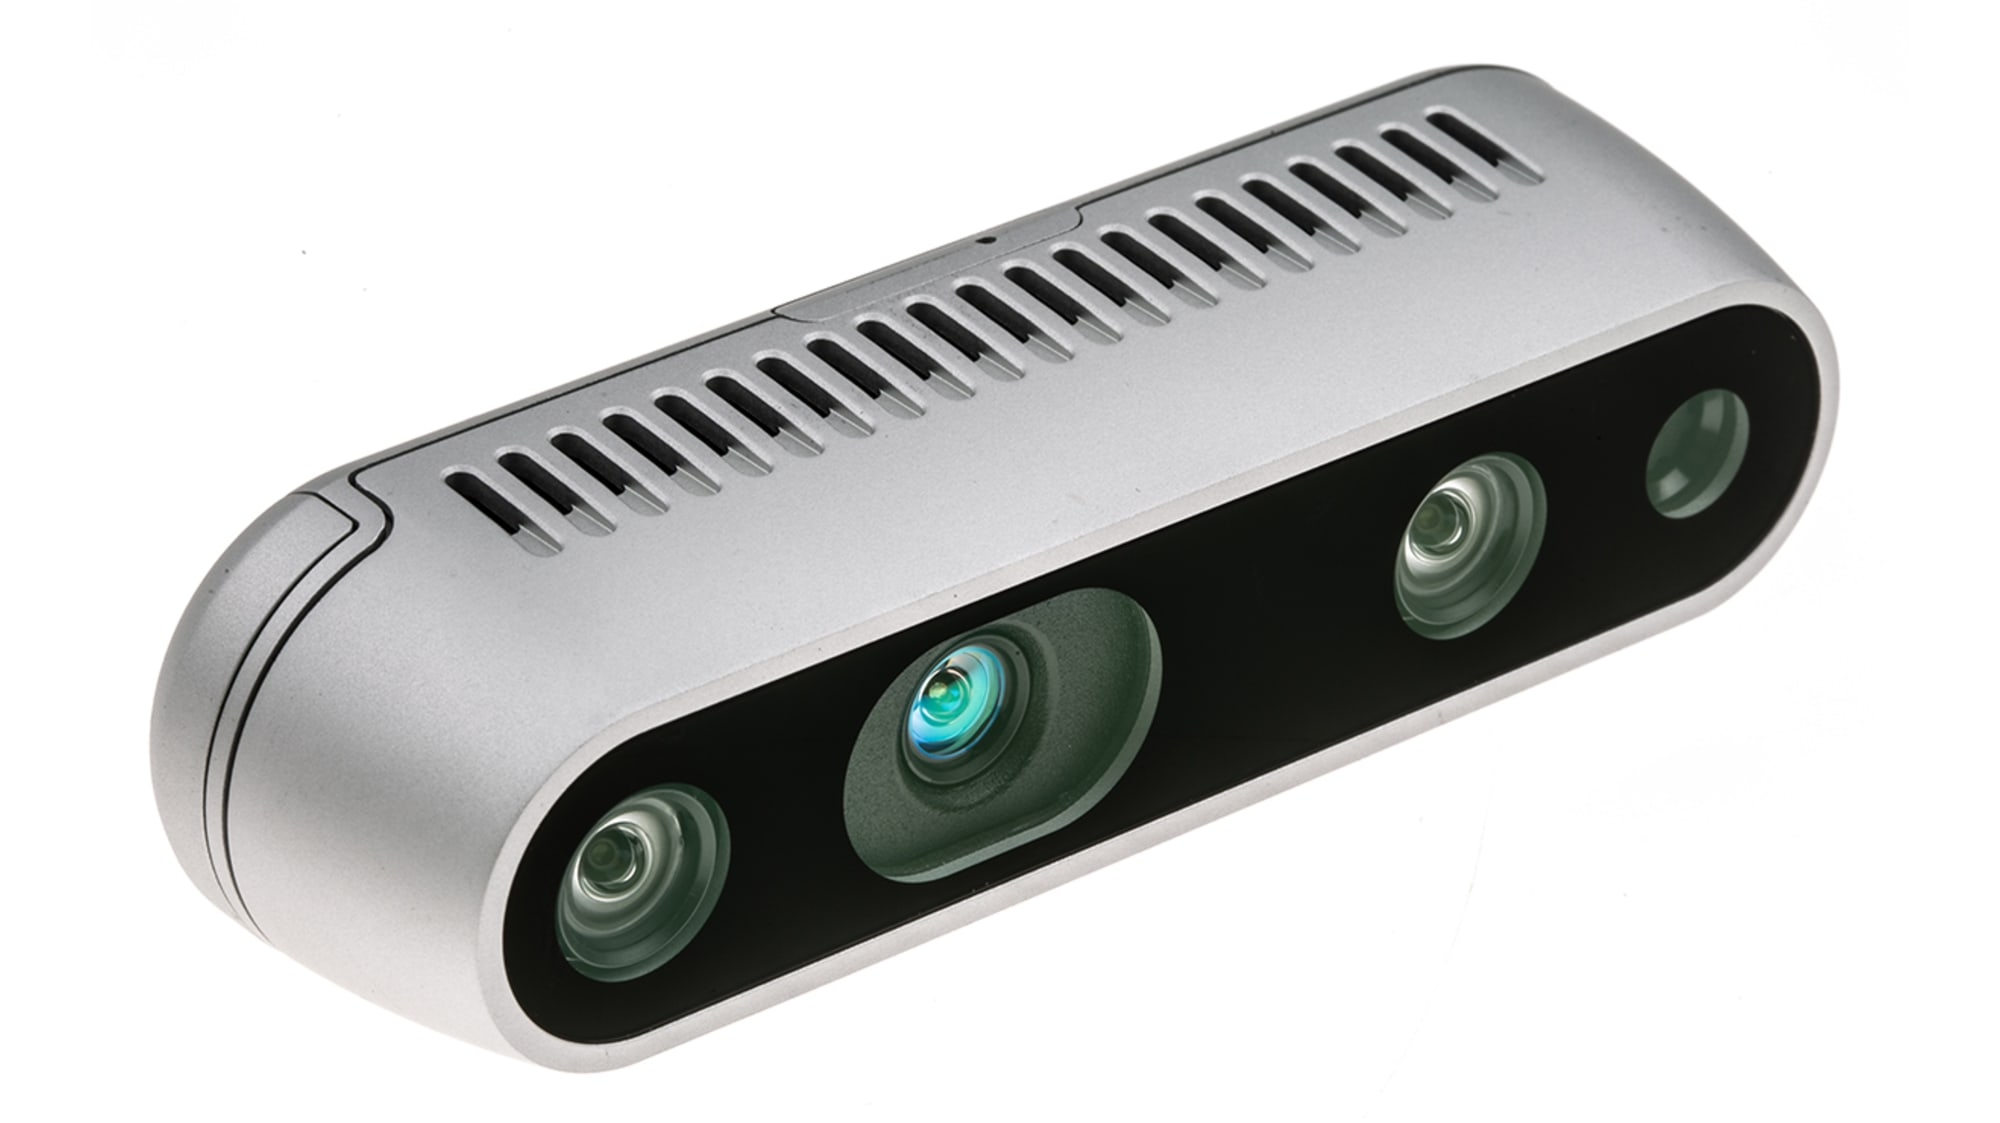
\includegraphics[scale=0.1]{figs/chapter3/d435i.jpg}
    \caption{Intel RealSense D435i stereo depth camera.}
    \label{fig:d435i}
\end{figure}

\newsubsection{Computer di bordo}
\indent La restante parte dell'elettronica è costituita dal computer di bordo. Si tratta in questo caso di un calcolatore di più alto livello, dedicato allo svolgimento dei task più lenti di supervisione e decisione, nonché ai compiti di processamento più onerosi per ottenere una stima precisa della posa locale, implementando le logiche di navigazione.\\
Le piattaforme Nvidia Jetson sono state selezionate per questo scopo, in quanto soluzioni SoC altamente efficienti e dotate di svariato hardware integrato, predisposte anche per lo sviluppo di software di qualunque tipo grazie al supporto del sistema operativo Linux. Il modello specifico che è stato adottato è la development board Xavier NX, rappresentata in Figura \ref{fig:nx}. La principale caratteristica di queste soluzioni è l'ampia e varia disponibilità di risorse in un package di dimensioni e consumi contenuti. Le caratteristiche salienti e più utili ai fini del presente lavoro sono riassunte nella Tabella \ref{tab:nx}.
\vspace{0.5cm}
\begin{table}[h]
    \centering
    \begin{tabular}{c|c}
        \textbf{CPU} & 6-core NVIDIA Carmel ARM v8.2 64-bit\\
        \textbf{GPU} & NVIDIA Volta architecture, 384 CUDA cores, CUDA 10.1\\
        \textbf{RAM} & 8 GB 128-bit LPDDR4x\\
        \textbf{Interfacce} & Gigabit Ethernet, WiFi, Bluetooth, GPIO, I2C/S, SPI, UART, USB
    \end{tabular}
    \caption{Caratteristiche tecniche del SoC Nvidia Jetson Xavier NX.}
    \label{tab:nx}
\end{table}

\begin{figure}
    \centering
    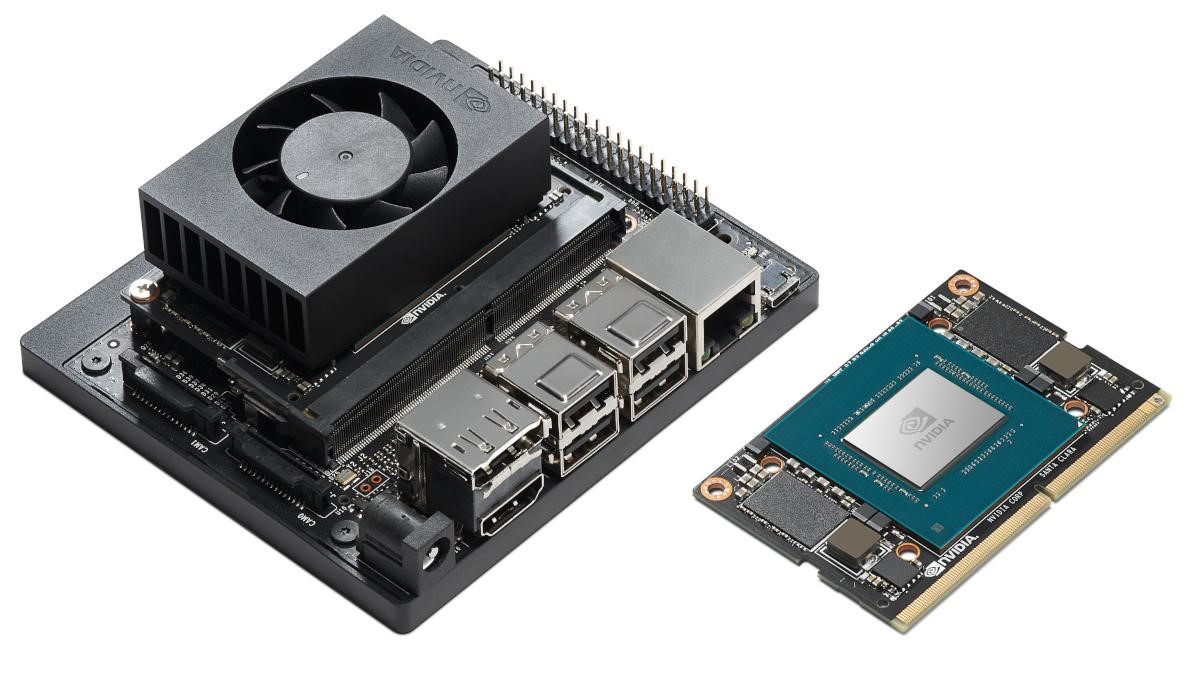
\includegraphics[scale=0.35]{figs/chapter3/nx.jpg}
    \caption{SoC Nvidia Jetson Xavier NX.}
    \label{fig:nx}
\end{figure}

\newsection{Operating System}
\indent Appare chiaro dall'architettura illustrata finora come in questo progetto si sia reso necessario interagire con l'hardware, a basso livello, e contemporaneamente sviluppare un software stratificato che lo pilotasse e implementasse opportune logiche decisionali. Per far questo, è apparsa da subito chiara la necessità di un sistema operativo che consentisse di operare facilmente ad ogni livello. Le soluzioni Jetson, basate su architettura ARM, sono studiate per essere utilizzate con il sistema operativo Linux, che soddisfa totalmente tali requisiti operativi. Ciò nonostante, è stato necessario un lavoro di configurazione ad-hoc a partire dall'installazione fornita da Nvidia per meglio adattarla al presente caso d'uso e consentire l'integrazione del resto dell'hardware e degli strumenti software impiegati.\\
L'installazione di default offerta da Nvidia è costituita dalla distribuzione Ubuntu Linux 18.04 con kernel 4.9 PREEMPT\footnote{La versione PREEMPT del kernel Linux è caratterizzata da latenze ridotte, in quanto fatta eccezione per alcune sezioni molto critiche esso risulta sempre interrompibile.}, racchiusa in una collezione di package denominata \emph{Linux 4 Tegra}. Si tratta di un'installazione stabile e testata, dotata di un set di pacchetti e librerie più limitato rispetto alle versioni base ma di tutti i driver necessari ad usare l'hardware presente sulla board. La prima strada intrapresa è stata quella dell'aggiornamento a Ubuntu 20.04, ancora non standardizzata da Nvidia, lungo la quale sono sorti diversi problemi legati all'aggiornamento delle librerie grafiche pian piano risolti. Successivamente, allo scopo di aumentare ancora di più la responsività e la predicibilità del sistema, è stata tentata la costruzione di un'installazione stabile con kernel 4.9 PREEMPT RT\footnote{La versione PREEMPT RT del kernel, ottenuta mediante l'applicazione di un set di patches prima della compilazione, è caratterizzata dall'interrompibilità totale in qualunque punto e dall'assenza di primitive di sincronizzazione di tipo \emph{locking}.}. Nonostante ripetuti tentativi di ricompilazione del kernel e di aggiornamento del sistema, sono sempre stati rilevati dei problemi di compatibilità con i driver e le librerie offerti da Nvidia, e gli incrementi prestazionali ricavati sono stati giudicati eccessivamente ridotti; oltre a ciò, si sospetta che l'aver reso interamente interrompibili anche i driver della GPU abbia reso meno efficienti alcuni algoritmi implementati su di essa. Per tali ragioni questa strada è stata abbandonata, e l'installazione PREEMPT è stata consolidata con delle performance accettabili sia sul fronte della varianza dei timer ad alta risoluzione, sia su quello dell'affidabilità delle schedulazioni soft real-time implementate mediante lo scheduler di sistema. Si ritiene, come si mostrerà, che un tale sistema sia adatto anche all'implementazione di loop di controllo veloci con campionamenti non inferiori al singolo millisecondo, naturalmente quando non si è complessivamente vicini ai suoi limiti di carico.\\
Per misurare le latenze e valutare le prestazioni complessive è stata impiegata la utility \emph{cyclictest}\footnote{https://wiki.linuxfoundation.org/realtime/documentation/howto/tools/cyclictest/start}, una cui esecuzione è mostrata a titolo di esempio nel listato seguente.
\vspace{1cm}
\begin{lstlisting}[language=bash, caption=Esempio di benchmark del SoC montato sul drone eseguito con la utility \emph{cyclictest}.]
nxdrone:~$ sudo cyclictest -m -p98 --smp
# /dev/cpu_dma_latency set to 0us
policy: fifo: loadavg: 0.33 0.61 0.32 1/381 10460          

T: 0 (10428) P:98 I:1000 C:   3365 Min:      7 Act:   30 Avg:   19 Max:     147
T: 1 (10431) P:98 I:1500 C:   2241 Min:      7 Act:   21 Avg:   22 Max:     294
T: 2 (10432) P:98 I:2000 C:   1680 Min:      8 Act:   16 Avg:   27 Max:     352
T: 3 (10434) P:98 I:2500 C:   1343 Min:      8 Act:   23 Avg:   22 Max:     155
T: 4 (10435) P:98 I:3000 C:   1118 Min:      7 Act:   30 Avg:   25 Max:     147
T: 5 (10436) P:98 I:3500 C:    958 Min:      9 Act:   22 Avg:   24 Max:     319
\end{lstlisting}

Da tale esecuzione si evince come le latenze siano comunque contenute, in media nell'ordine delle decine di microsecondi, con dei picchi attesi data la configurazione del sistema, dipendenti dal carico ma comunque mai eccessivi.
\clearpage

\newsection{Software}
\indent La realizzazione di un drone autonomo in grado di eseguire deterministicamente e con precisione i task specificati nel regolamento del Contest ha posto come prima problematica la scelta di un'architettura software efficiente, e anche comoda da usare sia durante lo sviluppo che in fase di testing. Per ragioni che a questo punto dovrebbero risultare evidenti, all'installazione di Linux descritta nella sezione precedente è stato aggiunto il middleware ROS 2 versione Foxy Fitzroy.\\
I vari task necessari al compimento di una missione sono stati suddivisi in livelli:
\begin{itemize}
    \item a basso livello: comunicazione con il controllore di volo Pixhawk per invio comandi, ricezione di feedback e informazioni di stato e campionamento dell'odometria;
    \item ad un livello intermedio: comunicazione con le camere per configurarle e ricevere i frame da cui estrarre informazioni;
    \item ad un livello più alto: algoritmi di esplorazione, navigazione e precision landing, logica decisionale e comunicazione con la Ground Control Station.
\end{itemize}
Ciascuno di questi moduli è stato realizzato come package ROS 2, comprendente uno o più nodi secondo le necessità. Ciò che li differenzia è la diversa modalità operativa: i nodi appartenenti al livello più basso hanno quasi sempre callbacks in esecuzione o eventi da gestire, e fanno un uso quasi esclusivo dei messaggi; quelli appartenenti al livello intermedio svolgono lavoro non appena sono disponibili nuovi dati da processare, pubblicando i risultati sempre sotto forma di messaggi; infine, le logiche e gli algoritmi di più alto livello sono attivati solo quando richiesto, ossia in momenti specifici della missione, e sono pertanto invocati sempre mediante dei servizi. Le interfacce che si è dovuto definire ad-hoc sono state raccolte nel package \emph{afg\_interfaces}, mentre quelle proprie di PX4 si possono trovare nel package \emph{px4\_msgs}\footnote{https://github.com/PX4/px4\_msgs}. L'implementazione corretta del microRTPS Bridge è stata raccolta in un fork del package \emph{px4\_ros\_com}\footnote{https://github.com/Automazione-Tor-Vergata/px4\_ros\_com}. Data la criticità di alcune operazioni, nonché la necessità di lavorare talvolta a diretto contatto con l'hardware a disposizione, l'unico linguaggio di programmazione impiegato è stato il C++. Nel resto di questa sezione si procederà dunque a descrivere nel dettaglio tutti i packages e i nodi che compongono l'architettura, secondo il naturale ordinamento gerarchico appena illustrato. Una rappresentazione complessiva di tale architettura è offerta in Figura \ref{fig:nodesgraph}: lo schema è stato ricavato con il tool rqt\_graph\footnote{Questo tool talvolta non esclude alcuni elementi interni al middleware dai diagrammi, dunque in alcuni di essi figureranno nodi o topic propri di ROS 2 o RQt stesso.} ed evidenzia tutti i nodi attivi sul drone e la GCS, nonché i topic su cui alcuni di essi si scambiano messaggi. Sono assenti i servizi, non rappresentabili graficamente dal tool, nonché i topic esposti dal microRTPS Agent su cui viaggiano le comunicazioni da e verso il controllore di volo: tutti questi elementi saranno illustrati più chiaramente nel seguito.\\
Ciascuno dei moduli che compongono questa architettura offre, sia all'operatore che agli altri moduli, un set di comandi invocabili mediante richieste ad opportuni servizi. Per testare singolarmente le varie unità senza il controllo della logica di supervisione, sono stati redatti svariati alias e funzioni per la shell Bash al fine di semplificare l'impiego dei comandi del middleware nei vari casi; un esempio è mostrato nel Listing \ref{lst:fcsetp}.

\begin{figure}
    \centering
    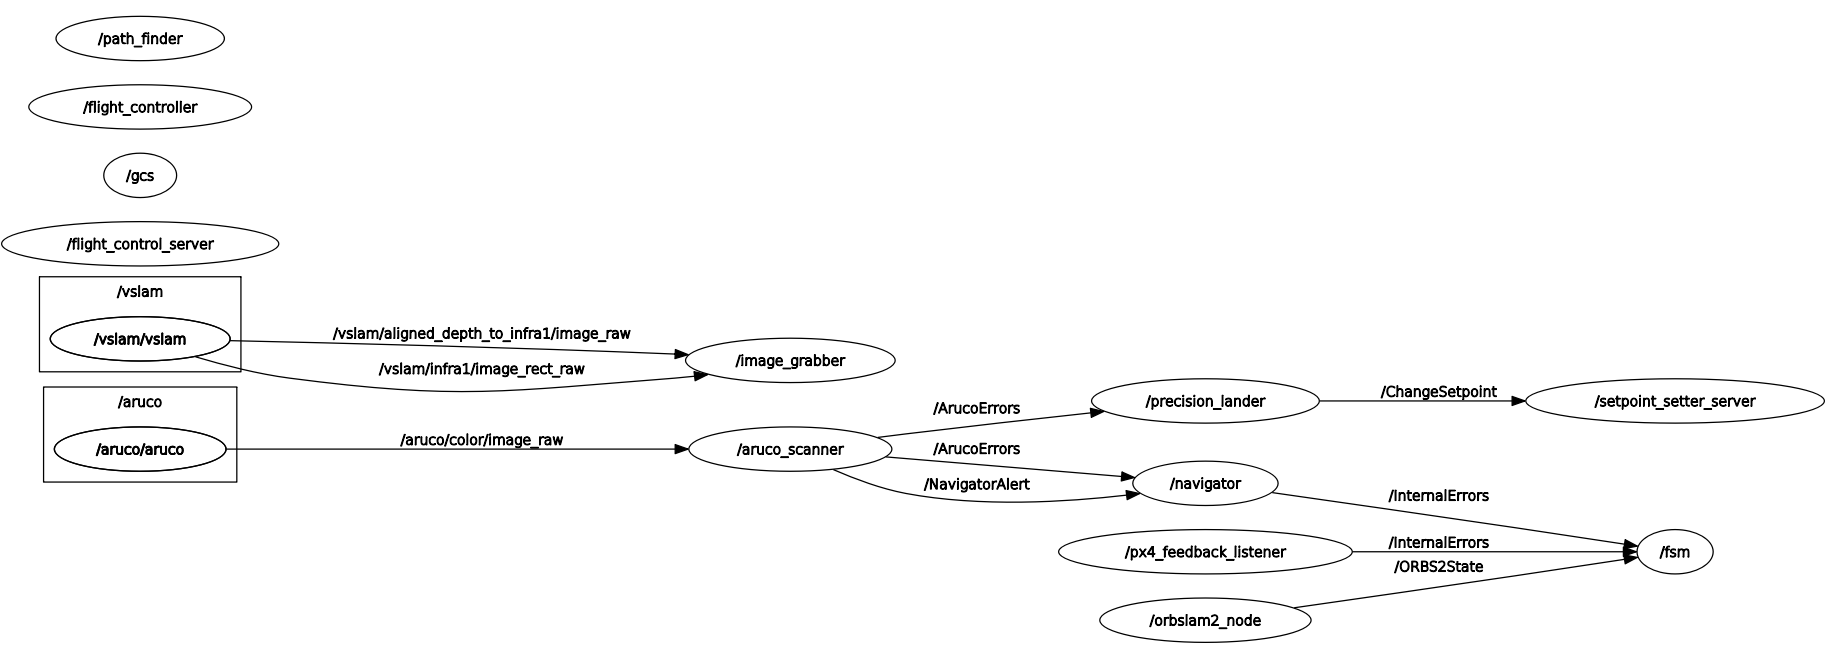
\includegraphics[width=\textwidth]{figs/chapter3/nodesgraph.png}
    \caption{Schema complessivo di nodi e topic attivi su drone e GCS.}
    \label{fig:nodesgraph}
\end{figure}
\vfill\newpage

\begin{lstlisting}[language=bash, caption={Esempio di funzione Bash per cambiare setpoint di posizione corrente.}, label={lst:fcsetp}]
# Routine to set a position setpoint
function fc_setp_pos {
    if [[ $# -ne 4 ]]; then
        echo "Usage:" 1>&2
        echo "    fc_setp_pos X Y Z YAW" 1>&2
        return 1
    fi
    ros2init
    ros2 service call /SetpointSetter afg_interfaces/srv/SetpointSetter\
    "{setpoint_conf: 0, x: $1, y: $2, z: $3, yaw: $(degrad $4)}"
}
\end{lstlisting}

\newsubsection{Flight Control}
\indent Il primo livello dell'architettura software, direttamente al di sopra del firmware PX4 in esecuzione nel controllore di volo Pixhawk, è rappresentato dal package \emph{Flight Control}. I compiti svolti da questo programma possono essere riassunti come segue, e sono stati ripartiti tra un totale di quattro nodi esattamente nello stesso modo:
\begin{itemize}
    \item invio di comandi a PX4 per l'esecuzione di operazioni relative al volo quali armamento, disarmamento, decollo e atterraggio, quando richiesto da altri nodi o da un operatore;
    \item invio periodico a PX4 di setpoint di posizione o velocità da inseguire;
    \item parsing delle richieste formulate dagli altri nodi per cambiare i setpoint da inviare a PX4, al fine di spostare il drone nell'ambiente;
    \item ricezione e parsing di feedback da PX4 relativi ai comandi operativi, nonché allo stato di basso livello del drone, e degli stessi messaggi di log di PX4.
\end{itemize}
Una rappresentazione completa di nodi e topic relativi a questo package è mostrata in Figura \ref{fig:fctrl}, mentre i listati seguenti espongono la struttura di ciascuno.
\newpage

\begin{lstlisting}[language={C++}, caption={Definizione del nodo \emph{flight\_controller}.}, label={lst:fcontroller}]
class FlightController : public rclcpp::Node
{
public:
    FlightController();

private:
    rclcpp::Publisher<TrajectorySetpoint>::SharedPtr traj_setpoint_pub_;
    rclcpp::Publisher<OffboardControlMode>::SharedPtr offboard_cmode_pub_;
    rclcpp::CallbackGroup::SharedPtr setpoints_clbk_group_;
    rclcpp::TimerBase::SharedPtr setpoint_pub_timer_;

    void setpoint_timer_clbk(void);
};
\end{lstlisting}

\vspace{3cm}

\begin{figure}[h!]
    \centering
    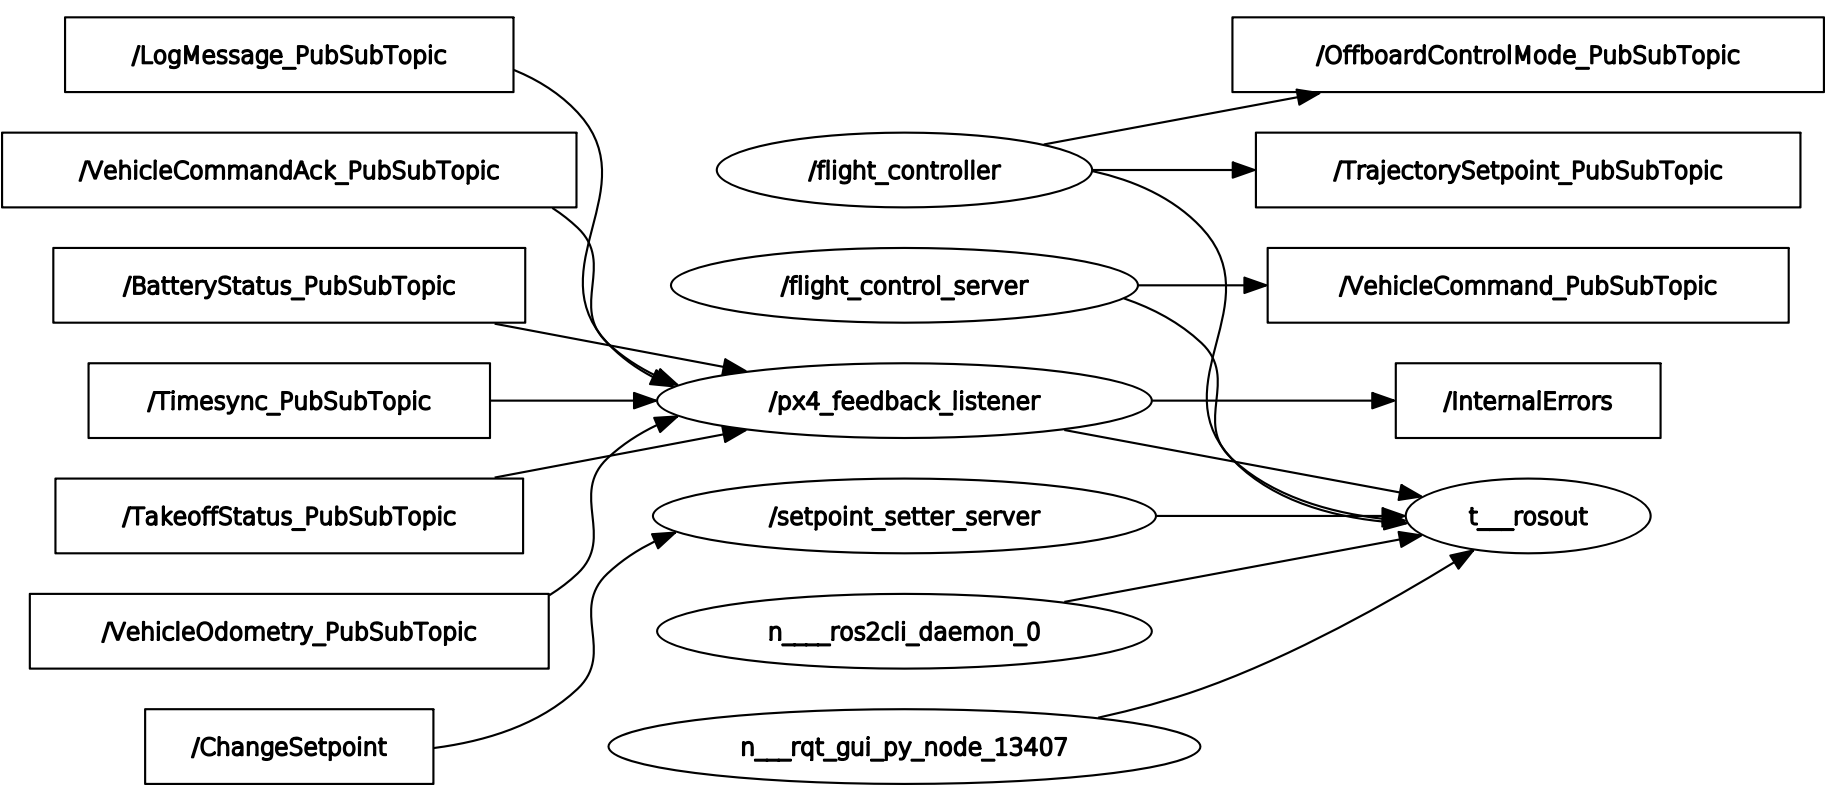
\includegraphics[width=\textwidth]{figs/chapter3/fctrl.png}
    \caption{Schema riassuntivo di nodi e topic del package \emph{Flight Control}.}
    \label{fig:fctrl}
\end{figure}
\clearpage

\begin{lstlisting}[language=C++, caption={Definizione del nodo \emph{control\_server}.}, label={lst:ctrlserver}]
class ControlServer : public rclcpp::Node
{
public:
    ControlServer();

    void arm(FlightControl::Response::SharedPtr resp) const;
    void disarm(FlightControl::Response::SharedPtr resp) const;
    void takeoff(FlightControl::Response::SharedPtr resp) const;
    void land(FlightControl::Response::SharedPtr resp) const;
    void manual_on(FlightControl::Response::SharedPtr resp) const;
    void manual_off(FlightControl::Response::SharedPtr resp) const;
    void setp_on(FlightControl::Response::SharedPtr resp) const;
    void setp_off(FlightControl::Response::SharedPtr resp) const;
    void reset(FlightControl::Response::SharedPtr resp) const;

private:
    rclcpp::Publisher<VehicleCommand>::SharedPtr vehicle_cmd_pub_;
    rclcpp::Service<FlightControl>::SharedPtr flight_control_srv_;
    rclcpp::CallbackGroup::SharedPtr flight_control_clbk_group_;

    uint16_t publish_vehicle_cmd(uint16_t cmd,
                                 float p1 = NAN,
                                 float p2 = NAN,
                                 float p3 = NAN,
                                 float p4 = NAN,
                                 float p5 = NAN,
                                 float p6 = NAN,
                                 float p7 = NAN) const;
    void flight_control_clbk(const FlightControl::Request::SharedPtr request,
                             const FlightControl::Response::SharedPtr response);
};
\end{lstlisting}
\clearpage

\begin{lstlisting}[language=C++, caption={Definizione del nodo \emph{setpoint\_server}.}, label={lst:setpserver}]
class SetpointServer : public rclcpp::Node
{
public:
    SetpointServer();

    bool change_target_setpoint(uint8_t conf,
                                float x,
                                float y,
                                float z,
                                float vx,
                                float vy,
                                float vz,
                                float yaw);

private:
    rclcpp::Service<SetpointSetter>::SharedPtr setpoint_set_srv_;
    rclcpp::Subscription<ChangeSetpoint>::SharedPtr setpoint_set_sub_;
    rclcpp::CallbackGroup::SharedPtr setpoint_msg_clbk_group_;
    rclcpp::CallbackGroup::SharedPtr setpoint_srv_clbk_group_;

    void setpoint_set_srv_clbk(const SetpointSetter::Request::SharedPtr request,
                               const SetpointSetter::Response::SharedPtr response);
    void setpoint_set_msg_clbk(const ChangeSetpoint::SharedPtr msg);
};
\end{lstlisting}
\clearpage

\begin{lstlisting}[language=C++, caption={Definizione del nodo \emph{px4\_feedback\_listener}.}, label={lst:pflistener}]
class PX4FeedbackListener : public rclcpp::Node
{
public:
    PX4FeedbackListener();

private:
    rclcpp::Subscription<VehicleCommandAck>::SharedPtr vehicle_cmd_ack_sub_;
    rclcpp::Subscription<TakeoffStatus>::SharedPtr takeoff_status_sub_;
    rclcpp::Subscription<BatteryStatus>::SharedPtr battery_status_sub_;
    rclcpp::Subscription<Timesync>::SharedPtr timesync_sub_;
    rclcpp::Subscription<LogMessage>::SharedPtr log_message_sub_;
    rclcpp::Subscription<VehicleOdometry>::SharedPtr odometry_sub_;

    rclcpp::CallbackGroup::SharedPtr vehicle_cmd_ack_clbk_group_;
    rclcpp::CallbackGroup::SharedPtr takeoff_status_clbk_group_;
    rclcpp::CallbackGroup::SharedPtr battery_status_clbk_group_;
    rclcpp::CallbackGroup::SharedPtr timesync_clbk_group_;
    rclcpp::CallbackGroup::SharedPtr log_message_clbk_group_;
    rclcpp::CallbackGroup::SharedPtr odometry_clbk_group_;

    rclcpp::Publisher<InternalError>::SharedPtr error_pub_;

    rclcpp::Clock clock_ = rclcpp::Clock(RCL_STEADY_TIME);
    rclcpp::Time low_bat_timer_ = rclcpp::Time(0, 0, RCL_STEADY_TIME);

    void vehicle_cmd_ack_msg_clbk(const VehicleCommandAck::SharedPtr msg);
    void takeoff_status_msg_clbk(const TakeoffStatus::SharedPtr msg);
    void battery_status_msg_clbk(const BatteryStatus::SharedPtr msg);
    void timesync_msg_clbk(const Timesync::SharedPtr msg);
    void log_message_clbk(const LogMessage::SharedPtr msg);
    void odometry_msg_clbk(const VehicleOdometry::SharedPtr msg);
};
\end{lstlisting}
\clearpage

PX4 offre diverse modalità di volo, sia automatico che manuale; ai fini di questo lavoro quelle d'interesse sono le seguenti:
\begin{itemize}
    \item \textbf{MANUAL:} In questa modalità il drone è totalmente sotto il controllo del pilota, che può operare mediante un normale radiocomando la cui ricevente deve essere collegata al Pixhawk. Per questo progetto si è usato un radiocomando FrSky Taranis.
    \item \textbf{OFFBOARD:} È la modalità di volo automatico standard, durante la quale si presuppone che il controllore di volo debba pilotare il drone in modo da eseguire dei comandi impartiti da un companion PC montato a bordo. Tali comandi sono dei setpoint di posizione nello spazio e angolo di yaw, oppure di velocità lineare e di imbardata e angolo di yaw; affinché il controllore di volo ritenga stabile la comunicazione col companion PC e non entri in failsafe, i setpoint devono essere inviati in continuazione ad un rate il più possibile stabile e superiore a 2 Hz. L'inserimento di questa modalità deve avvenire successivamente all'armamento e porta il drone a decollare verso il setpoint corrente.
    \item \textbf{LAND:} Non appena viene inserita questa modalità, presupponendo che il drone sia in volo, viene iniziata una discesa verticale stabilizzata verso il suolo. Un modulo interno a PX4 noto come \emph{Land Detector}, e che consiste essenzialmente in una macchina a stati, si occupa di regolare la spinta e integrare le misure dell'odometria per capire quando il drone ha toccato terra e si è fermato, ossia può considerarsi atterrato.
\end{itemize}
Il Flight Control è stato pensato per essere una sorta di radiocomando a disposizione dei moduli di più alto livello, che consentisse di sfruttare le funzionalità sopracitate assicurando al contempo la possibilità di inserire prontamente il controllo manuale in caso di problemi. Per garantire la massima efficienza il package è stato programmato in modo concorrente, ripartendo le diverse callbacks su più thread e minimizzando l'uso di lock.\\
Alla base di tutto vi è il nodo \emph{flight\_controller}, la cui struttura è esposta nel Listing \ref{lst:fcontroller}. Il suo compito è semplicemente quello di postare un setpoint verso PX4 sul topic \emph{/TrajectorySetpoint}, e il tipo di setpoint tra quelli prima descritti sul topic \emph{/OffboardControlMode}, mediante opportuni publishers. Tale operazione è invocata da un timer, attraverso il quale si può impostare la frequenza di pubblicazione dei setpoint che è stata fissata a 20 Hz.\\
Il setpoint corrente può essere cambiato inviando una opportuna richiesta al nodo \emph{setpoint\_server}, descritto nel Listing \ref{lst:setpserver}. Tale nodo offre due modi per farlo: velocemente ma senza feedback sulla riuscita dell'operazione, inviando un messaggio contenente il nuovo setpoint sul topic \emph{/ChangeSetpoint}, oppure più lentamente ma con feedback formulando una richiesta al servizio \emph{/SetpointSetter}. In entrambi i casi viene invocata la routine \emph{change\_target\_setpoint}, la quale controlla la correttezza del setpoint richiesto e solo in caso positivo lo inserisce nel sistema. Il servizio \emph{/SetpointSetter} offre anche la possibilità di aggiornare il setpoint corrente con uno di posizione ed attendere che questo sia effettivamente raggiunto, eventualmente anche con l'assetto stabilizzato. Per ottenere questo effetto la callback del servizio controlla l'odometria postata da PX4, e ritorna una risposta solo quando il drone si trova entro una sfera attorno al setpoint, il cui raggio è pure specificabile nella richiesta, ha l'angolo di yaw prossimo a quello richiesto ed eventualmente quelli di roll e pitch sufficientemente limitati. Naturalmente tutte queste soglie, come un'infinità di altri parametri da cui dipende il funzionamento di questo package, sono stati definiti nel suo header file e tarati opportunamente. Sempre per massimizzare l'efficienza e consentire il raggiungimento di rate di pubblicazione anche molto elevati, i dati globali condivisi tra gli ultimi due nodi in cui sono codificati i setpoint da postare sono gestiti secondo uno schema lock-free, in cui la concorrenza è risolta mediante i tipi atomici di C++ e un uso opportuno dei \emph{memory orders} per indicare ai sottosistemi di CPU, cache e controller delle memorie quando e come eseguire le singole operazioni di lettura e scrittura ad essi relative. Tale meccanismo si è dimostrato molto efficiente ed è stato pertanto applicato più volte in situazioni simili presentatesi nel resto del software.\\
Andando già verso un livello leggermente più alto si incontra il nodo \emph{control\_server}, illustrato nel Listing \ref{lst:ctrlserver}. Il suo compito è offrire al resto dell'architettura un modo semplice di cambiare lo stato del drone, eseguendo le operazioni di base quali armamento, disarmamento, decollo e atterraggio. L'interfaccia con l'esterno è rappresentata dal servizio \emph{/FlightControl}, mediante cui ciascuna di tali operazioni può essere eseguita formulando una opportuna richiesta; in caso d'errore, la risposta riporterà lo stesso codice d'errore ritornato da PX4. Come si evince da listato, ciascuna operazione è codificata in una specifica routine invocata selettivamente dalla callback del servizio, che si risolve sempre nella pubblicazione di un messaggio verso PX4 sul topic \emph{/VehicleCommand} costruito nella routine \emph{publish\_vehicle\_command}. Gli ACK dei vari comandi inviati, nonché lo stato dell'esecuzione delle operazioni richieste, vengono opportunamente tracciati mediante altri topic su cui pubblica PX4 ed utilizzati per capire se l'operazione ha avuto successo o meno e si può restituire una risposta. Le logiche d'invio dei comandi prevedono anche tentativi di trasmissione multipli e timeouts per far fronte ad eventuali problemi del link seriale o del microRTPS Bridge. Vi è poi tutta una serie di routine destinate ad essere invocate tramite richieste formulate da un operatore in fase di testing, quali ad esempio la configurazione del Flight Control per la selezione delle modalità di volo tramite radiocomando, l'attivazione dello stream di setpoint pubblicati verso PX4, o il reset dello stato interno del modulo.\\
La realizzazione di quest'ultimo nodo si è resa necessaria fin da subito, in quanto anche il semplice inserimento di una modalità richiede la costruzione di un messaggio per PX4 dal formato poco intuitivo, e per controllare l'esito dell'operazione c'è bisogno di analizzare i messaggi in transito su altri topic nonché tenere traccia di quale sia inizialmente lo stato del drone stesso. Per questi motivi, e per come è codificato, il Flight Control si configura come una piccola macchina a stati finiti di limitata complessità, ma che appare all'esterno come un unico servizio con cui richiedere al controllore di volo operazioni di base formulando semplicissime richieste ROS. Costruire un modulo del genere, che rendesse semplice pilotare automaticamente il drone, è stato il primo problema ad essere affrontato e poi risolto grazie a ROS 2, ponendo le basi per il resto dell'architettura.\\
Tutti i feedback ricevuti da PX4, assieme alle misure in tempo reale dell'odometria da esso pubblicate, sono raccolti dal nodo \emph{px4\_feedback\_listener}, illustrato nel Listing \ref{lst:pflistener}. Il nodo dispone di diversi subscribers relativi ai seguenti topic:
\begin{itemize}
    \item \textbf{/VehicleCommandAck:} Ogni volta che un comando operativo viene postato a PX4, l'esito dell'operazione viene scritto in uno di questi messaggi.
    \item \textbf{/TakeoffStatus:} Le macchine a stati interne di PX4 pubblicano messaggi su questo topic ogni volta che il drone viene armato, fatto decollare, portato a terra o disarmato; questi messaggi assieme a quelli del punto precedente vengono dunque usati per capire se un decollo o un atterraggio sono andati a buon fine, attraverso un meccanismo di segnalazione tra thread basato su condition variables che coinvolge le callbacks di questi subscribers e quella del servizio /FlightControl.
    \item \textbf{/BatteryStatus:} Da questi messaggi viene letta la tensione di batteria corrente, e se si rileva che essa si è mantenuta per un certo intervallo di tempo al di sotto di una soglia critica viene allertata la logica di livello superiore mediante un messaggio sul topic \emph{/InternalErrors}.
    \item \textbf{/Timesync:} PX4 posta in tempo reale il valore in microsecondi del suo orologio interno, il cui zero corrisponde all'istante di accensione; questo valore è condiviso tra tutti i nodi del package in quanto va inserito in tutti i messaggi da postare verso PX4.
    \item \textbf{/LogMessage:} PX4 integra un sistema di logging multilivello simile a quello del kernel Linux; di norma, i messaggi vengono scritti assieme agli altri dati in un log file memorizzato nel Pixhawk e che può essere scaricato al termine del volo, ma sono anche pubblicati su questo topic e dunque la relativa callback li stamperà a schermo in modo che l'operatore possa tenere traccia in tempo reale anche dell'operato e dello stato del controllore di volo.
    \item \textbf{/VehicleOdometry:} In questi messaggi, pubblicati solitamente ad una frequenza di 100 Hz, sono scritte le misure integrate dal filtro di Kalman EKF2 relative a posizione, velocità e assetto del drone sotto forma di un quaternione di orientamento; ai fini di questo package, vengono estratti solo la posizione e i tre angoli di Eulero.
\end{itemize}
I primi test condotti con il prototipo sono stati orientati alla verifica del funzionamento del sistema e dell'architettura fino a questo livello, dunque ad accertarsi che quanto sin qui illustrato funzionasse e che il drone si potesse far decollare, spostare ed atterrare in modo deterministico. Per una varietà di problemi tecnici sorti in varie fasi del progetto, conseguire questo obiettivo ha richiesto quattro dei sei mesi a disposizione, e le ultime criticità sono state individuate e risolte solo durante il secondo giorno di gara. È però con immensa soddisfazione che si sottolinea come, nonostante le altre numerose limitazioni strutturali e costruttive, da quel momento in poi il prototipo abbia volato in modo totalmente affidabile e preciso, senza necessità di alcun intervento umano.

\newsubsection{RealSense Node}
\indent Un altro package di fondamentale importanza per il funzionamento del sistema è quello che si occupa di configurare le due camere Intel RealSense D435i ed esporle al resto dell'architettura. Trattandosi di soluzioni naturalmente orientate all'ambito della robotica, Intel distribuisce apertamente un package ROS 2 che comprende dei driver Linux per le camere RealSense, il cui funzionamento non è sempre affidabile ma ai fini di questo progetto è stato giudicato sufficientemente buono. L'eseguibile generato a partire da tale package può essere configurato in fase di avvio, usando opportuni launch files inclusi, per creare un nodo per ogni camera collegata, configurandola opportunamente e attivando o disattivando i vari sensori. Nel caso in esame la camera frontale, denominata \emph{vslam}, è stata configurata attivando il sensore a infrarossi e quello di profondità, mentre a quella inferiore denominata \emph{aruco} è stato attivato solo il sensore RGB per ottenere delle immagini a colori di Roomba e piazzole. Il frame rate è stato impostato a 30 fps per entrambe le camere. Le immagini scattate e i dati degli altri sensori sono pubblicati dai nodi di questo package su dei topic opportunamente denominati, usando interfacce standard di ROS 2 e una policy di QoS best-effort. Lo schema riassuntivo della configurazione ottenuta con le due camere è mostrato in Figura \ref{fig:cameranodes}.

\begin{figure}
    \centering
    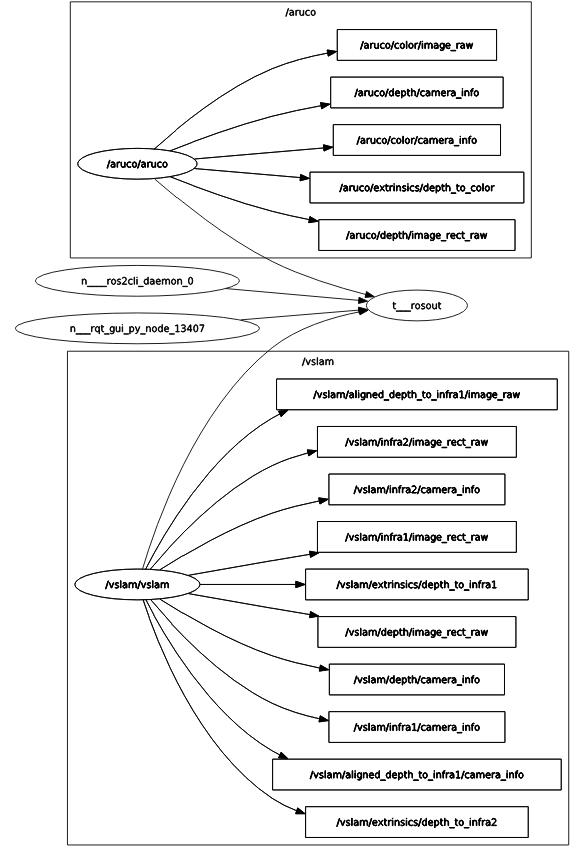
\includegraphics[width=0.7\textwidth]{figs/chapter3/cameranodes.png}
    \caption{Organizzazione di nodi e topic relativi alle due camere Intel RealSense.}
    \label{fig:cameranodes}
\end{figure}

\newsubsection{ORB\_SLAM2}
\indent Le regole del Contest prevedono che il drone non possa volare con l'ausilio di segnale GNSS, ma debba comunque localizzarsi nell'ambiente in tempo reale. Uno dei primissimi problemi da affrontare è stato proprio scegliere ed implementare sull'architettura costruita un algoritmo sufficientemente efficiente ed accurato, che potesse fornire a PX4 una stima attendibile e regolare della posa\footnote{Per \emph{posa} s'intende una combinazione di dati che esprimono la posizione nello spazio e l'orientamento di un corpo rigido.} locale. Il filtro di Kalman EKF2 può infatti essere configurato per volare senza GPS, escludendo completamente tale modulo ed affidandosi completamente ad altri metodi di localizzazione quali la visione artificiale, ma necessita di uno stream continuo di informazioni coerenti. Confrontando diverse soluzioni disponibili ed adeguatamente documentate, la scelta è ricaduta sul sistema di VSLAM\footnote{Tale sigla sta per "Visual Simultaneous Localization And Mapping", ed indica una classe di algoritmi basati sul riconoscimento di elementi all'interno di un'immagine al fine di mappare l'ambiente circostante un robot e localizzare quest'ultimo al suo interno in tempo reale.} ORB\_SLAM2. Si tratta della seconda versione del sistema ORB\_SLAM descritto in \cite{orbslam}, le cui estensioni rispetto alla versione originale sono elencate in \cite{orbslam2}. In sintesi, ORB\_SLAM2 si basa sull'estrazione di features binarie da un frame, sulla base delle quali viene man mano costruita una mappa locale. Le stesse features sono usate ovunque nel sistema in modo da evitare conversioni e massimizzare l'efficienza. I punti principali di una mappa locale, che ne costituiscono la parte essenziale, appartengono a un ristretto sottoinsieme di frames denominati \emph{keyframes}. I frame vengono incrociati per calcolare la posa locale corrente componendo un grafo chiamato \emph{Grafo di Covisibilità}, usato sia per localizzare il sistema che per costruire in memoria una mappa dell'ambiente. Man mano che la mappa cresce viene costruito un grafo che ne riassume le caratteristiche salienti, noto come \emph{Grafo Essenziale}, grazie al quale vengono individuati i loop; all'occorrenza del rilevamento di un loop viene effettuata una \emph{chiusura}: tutti i grafi vengono riesaminati e aggiornati, i keyframes e i nodi ridondanti vengono eliminati, e la mappa locale viene corretta in base ai rilevamenti fatti in modo da ridurre al minimo gli errori e renderla il più possibile coerente con la realtà. Per i dettagli teorici dietro il funzionamento di questo sistema si rimanda sempre a \cite{orbslam}. Dal punto di vista implementativo, tutto può essere fatto in real-time dato che ciascuna delle tre fasi di tracking, local mapping e loop closing descritte poc'anzi è affidata ad uno specifico thread. La versione 2 aggiunge un quarto thread, attivato subito dopo la chiusura di un loop, il cui compito è ripercorrere l'intera mappa al fine di apportare le dovute correzioni ed eliminare le ridondanze. L'organizzazione di questi thread è riassunta in Figura \ref{fig:orbthreads}. Altri miglioramenti apportati sono stati l'aggiunta del supporto alle camere stereo, come le RealSense impiegate in questo progetto, e lo sviluppo di una modalità chiamata \emph{localizzazione}, in cui il sistema carica all'avvio una mappa salvata su file e si limita a localizzarsi al suo interno, senza tentare di ottimizzarla o estenderla. In Figura \ref{fig:orbgraphs}, a titolo d'esempio, è rappresentata la costruzione dei grafi sopracitati ed un esempio di loop closure effettuate su uno dei dataset usati per testare la prima versione del sistema.\\
L'impiego di ORB\_SLAM2 si è dimostrato inizialmente problematico. Nonostante l'implementazione fornita di base dagli autori funzioni bene, si rileva facilmente da un'ispezione del codice e degli ottimizzatori di terze parti cui si appoggia come sia fortemente legata all'architettura x86, soprattutto in alcuni punti relativi all'estrazione ed elaborazione delle features, eseguite con istruzioni vettoriali AVX/SSE. Il passaggio all'architettura ARM ha richiesto di disabilitare queste ottimizzazioni, dato che l'alternativa sarebbe stata riscrivere i punti corrispondenti usando le istruzioni vettoriali NEON, cosa impossibile visti i tempi a disposizione. Si è invece apportato un miglioramento riscrivendo alcune parti del sistema per far uso della GPU montata sulla Jetson NX, attraverso istruzioni per l'architettura CUDA e l'uso della toolchain basata sul compilatore NVCC, e sfruttando al massimo le ottimizzazioni della toolchain GCC in fase di compilazione della libreria. Nonostante tutto, le performance ottenute sono complessivamente solo accettabili, ed un ulteriore lavoro di porting sarà necessario per costruire un'implementazione per ARM che possa considerarsi efficiente al pari della controparte x86. Questo parte è stato curata a più riprese in collaborazione con l'Ing. Fabrizio Romanelli, cui si devono anche altri sostanziali miglioramenti alla codebase di ORB\_SLAM2 relativi alla gestione della mappa, nonché una esaustiva spiegazione del funzionamento e delle modalità d'uso di questo sistema assieme alle camere RealSense.\\
Dato che l'esito di un qualunque volo dipende dal funzionamento di questo sistema, sono state tentate varie strade per trovare il modo migliore di utilizzarlo. Inizialmente è stata percorsa la strada della localizzazione: si è acquisita una mappa del campo gara, contenuta in un file grande un centinaio di MB, e la si è ricaricata a runtime sul drone al fine di fargliela usare per localizzarsi. Questo approccio ha avuto fin da subito due grossi problemi: nonostante la precisione con cui la mappa poteva essere acquisita, ci sarebbero sempre stati dei punti in cui il drone avrebbe fatto fatica a localizzarsi poiché poveri di features, e in tale modalità il sistema non ne avrebbe cercate di nuove; inoltre, dovendo processare in tempo reale una mappa globale di grandi dimensioni, la scarsa ottimizzazione per CPU ARM si faceva sentire sotto forma di rate di campionamento molto bassi, nell'ordine di 8-10 Hz, mentre si è sperimentato che PX4 richiede dati di posa a non meno di 16 Hz. A quest'ultima criticità si è tentato di far fronte implementando degli estrapolatori, dapprima quadratici e poi lineari, al fine di predire un campione in più da un buffer circolare di lunghezza fissa. Nonostante il drone fosse così in grado di volare abbastanza bene, la suscettibilità del sistema di localizzazione su mappa alle variazioni delle condizioni di luce hanno fatto optare per un ritorno al volo in SLAM puro. In questa modalità, tarando opportunamente il numero massimo di features da estrarre da un'immagine, è stato possibile ottenere rate di campionamento stabili e anche superiori ai 20 Hz; dopo aver riscontrato quale fosse il carico del resto del software, il numero massimo di features ottimale è stato individuato in 600 contro le 1000 di base, corrispondente ad un rate di circa 20 Hz a pieno carico. È stato necessario ridurre così tanto questo valore anche perché un rate di campionamento instabile corrisponde a dei frame spazialmente troppo distanti, dai quali si è riscontrato che il sistema estrae senza volerlo delle misure errate, con errori anche di svariate decine di centimetri che non è poi più in grado di correggere. Infine si è osservato che i tetti degli ostacoli del campo erano costruiti con un materiale traslucido, che causava riflessi nelle immagini visti come elementi in movimento assieme al drone, il quale tendeva dunque a correggere spostamenti che di fatto non aveva eseguito; la soluzione per ridurre questo effetto è stata montare la camera frontale su un supporto inclinato di 26.6° di pitch verso il basso. Così facendo si è ottenuto un sistema molto performante e preciso, reso ancora più affidabile dall'aggiunta di un filtro sulle misure di X, Y e Z che ne attenuasse le variazioni e ritardasse le correzioni apportate dal drone in caso di campioni spuri.\\
Il sistema ORB\_SLAM2 è usato attraverso il package ROS 2 \emph{orbslam2}, scritto sempre in collaborazione con l'Ing. Romanelli e composto da due nodi in esecuzione su un singolo thread, denominati rispettivamente \emph{image\_grabber} ed \emph{orbslam2\_node}. I listati seguenti ne illustrano la struttura, mentre nelle Figure \ref{fig:imgrabber} e \ref{fig:orb2node} è riportato un loro schema riassuntivo dal punto di vista del middleware.

\begin{figure}
    \centering
    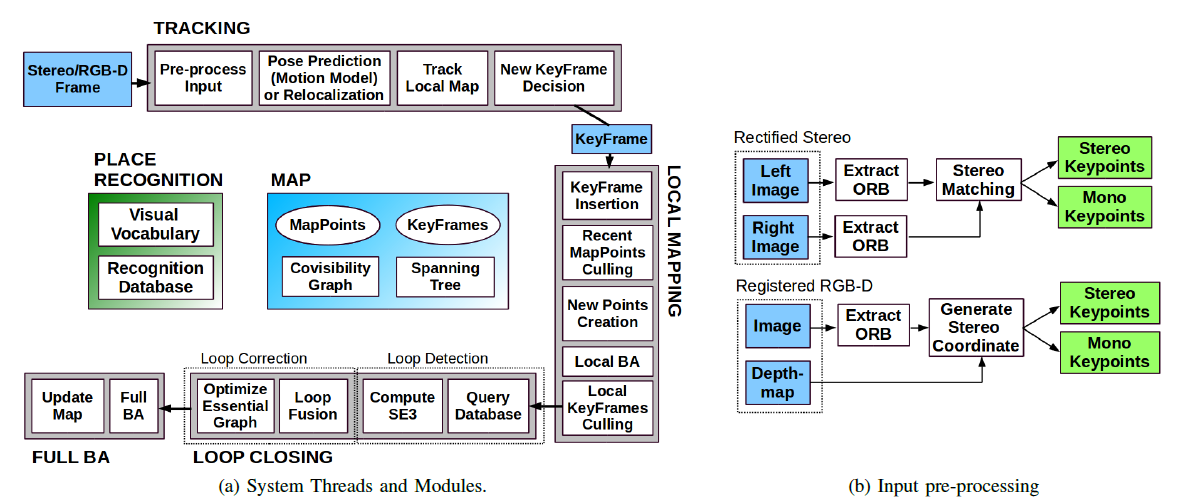
\includegraphics[width=\textwidth]{figs/chapter3/orbthreads.png}
    \caption{Organizzazione dei thread del sistema ORB\_SLAM2.}
    \label{fig:orbthreads}
\end{figure}

\begin{figure}
    \centering
    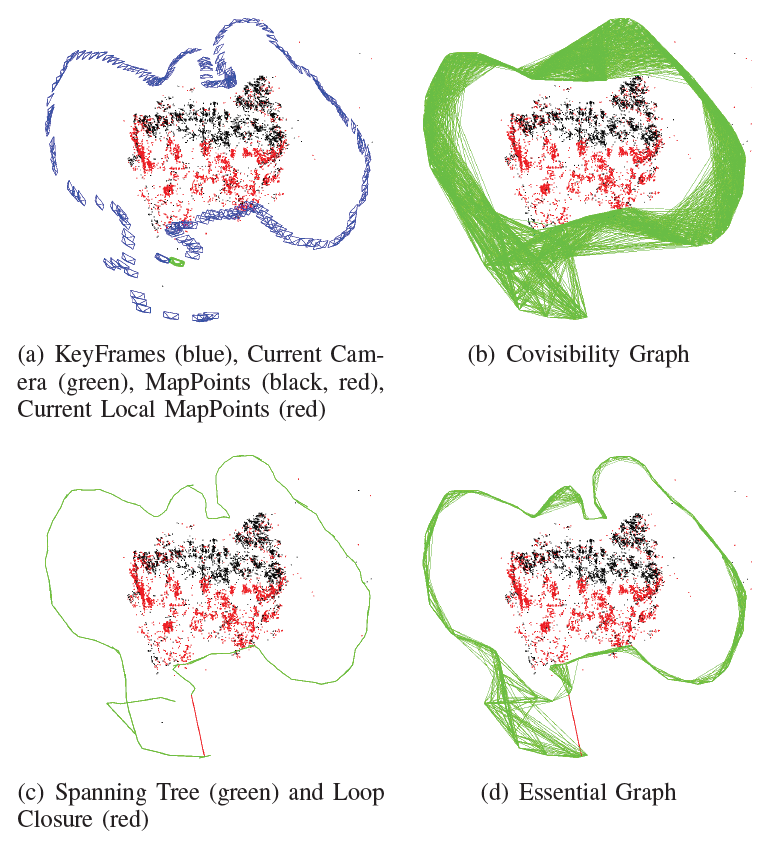
\includegraphics[width=0.6\textwidth]{figs/chapter3/orbgraphs.png}
    \caption{Costruzione dei grafi mediante frames e loop closure effettuate dal sistema ORB\_SLAM su uno dei dataset di test.}
    \label{fig:orbgraphs}
\end{figure}
\clearpage

\begin{figure}
    \centering
    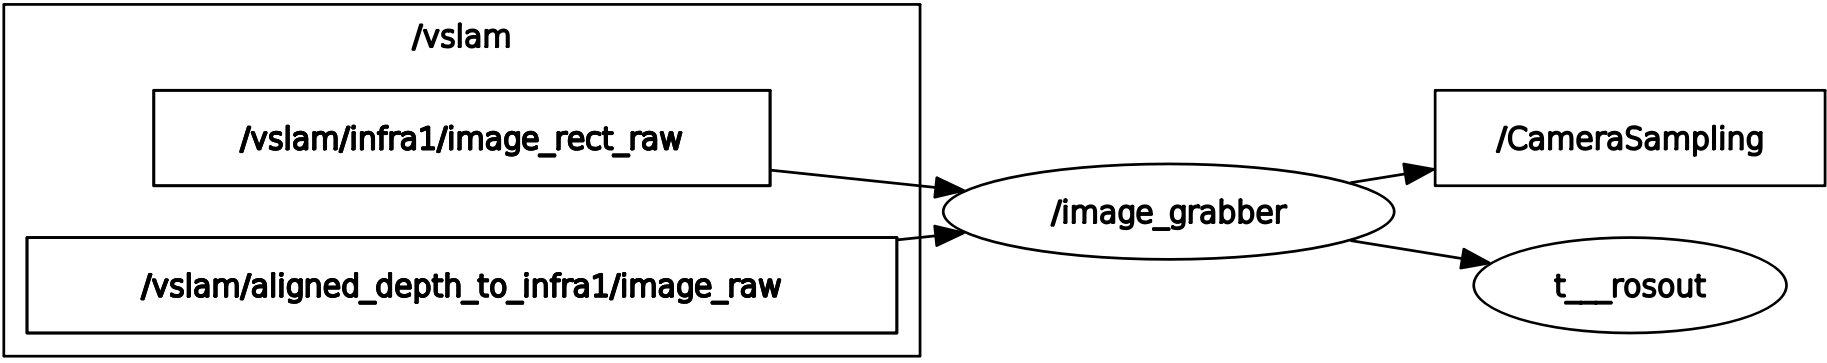
\includegraphics[width=0.7\textwidth]{figs/chapter3/imagegrabber.png}
    \caption{Organizzazione del nodo \emph{image\_grabber}.}
    \label{fig:imgrabber}
\end{figure}

\begin{figure}
    \centering
    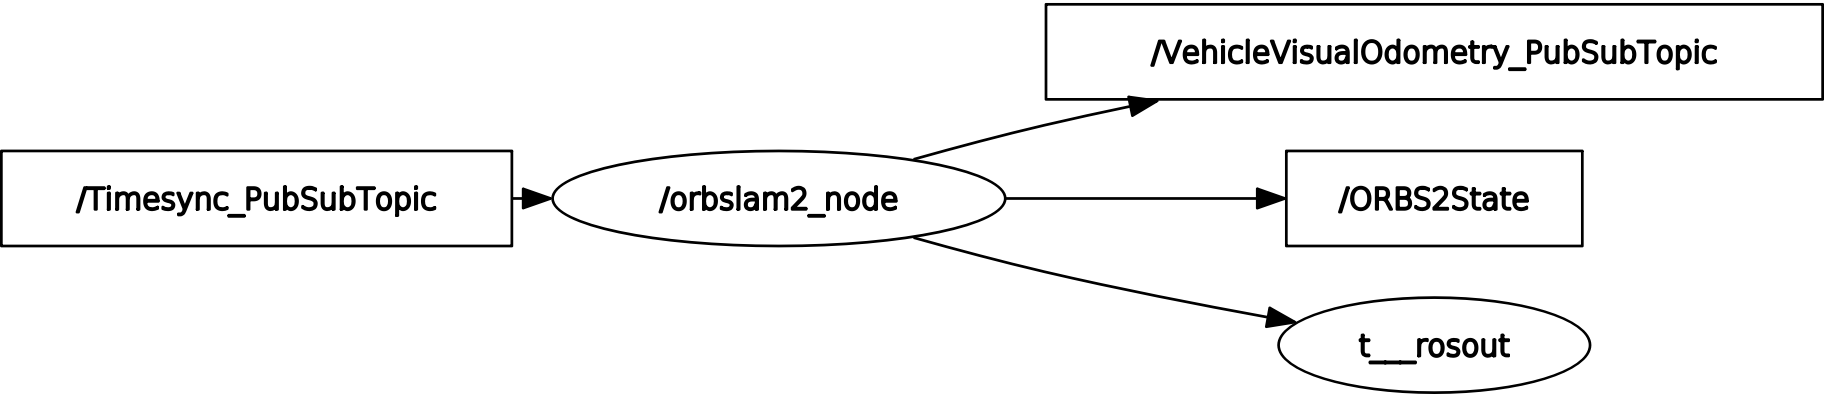
\includegraphics[width=0.7\textwidth]{figs/chapter3/orbslam2node.png}
    \caption{Organizzazione del nodo \emph{orbslam2\_node}.}
    \label{fig:orb2node}
\end{figure}

\begin{lstlisting}[language=C++, caption={Definizione del nodo \emph{orbslam2\_node}.}, label={lst:orb2node}]
class ORBSLAM2Node : public rclcpp::Node
{
public:
    ORBSLAM2Node(ORB_SLAM2::System *pSLAM,
                 ORB_SLAM2::System::eSensor _sensorType,
                 float camera_pitch,
                 int start_pad,
                 bool filter);

    void setPose(cv::Mat _pose);
    void setState(int32_t _state);

private:
    rclcpp::CallbackGroup::SharedPtr vio_clbk_group_;
    rclcpp::TimerBase::SharedPtr vio_timer_;
    rclcpp::Publisher<Int32>::SharedPtr state_publisher_;

    std::mutex poseMtx;
    std::mutex stateMtx;

    ORB_SLAM2::System *mpSLAM;
    ORB_SLAM2::System::eSensor sensorType;
    int32_t orbslam2State = ORB_SLAM2::Tracking::eTrackingState::SYSTEM_NOT_READY;

    cv::Mat orbslam2Pose = cv::Mat::eye(4, 4, CV_32F);
    float camera_pitch_;
    float cp_sin_, cp_cos_;
    int start_pad_;
    float x_offset_, y_offset_, z_offset_;
    bool filter_;

    const float a_0_ = 0.239018f;
    const float a_1_ = -0.7379f;
    const float b_0_ = 0.19080f;
    const float b_1_ = 0.31028f;
    const float tau_dynamic_thresh_[3] = {0.5f, 0.7f, 0.2f};
    const float tau_thresh_min_[3] = {0.1f, 0.1f, 0.08f};
    const float tau_dynamic_min_ = 0.1f;
    const float tau_dynamic_slow_ = 0.98f;

    float y_filtered_old_[3] = {0.0f, 0.0f, 0.0f};
    float y_filtered_old_old_[3] = {0.0f, 0.0f, 0.0f};
    float orb_data_old_[3] = {0.0f, 0.0f, 0.0f};
    float orb_data_old_old_[3] = {0.0f, 0.0f, 0.0f};
    float y_timevariant_old_[3] = {0.0f, 0.0f, 0.0f};
    float tau_dynamic_[3] = {0.0f, 0.0f, 0.0f};
    float orb_buffer_[3][8];

    void timer_vio_callback(void);

    void timestamp_callback(const Timesync::SharedPtr msg);

    float orb_filter(float sample, int axis);

    std::atomic<uint64_t> timestamp_;
    rclcpp::CallbackGroup::SharedPtr timestamp_clbk_group_;
    rclcpp::Publisher<VehicleVisualOdometry>::SharedPtr vio_publisher_;
    rclcpp::Subscription<Timesync>::SharedPtr ts_sub_;
};
\end{lstlisting}
\clearpage

\begin{lstlisting}[language=C++, caption={Definizione del nodo \emph{image\_grabber}.}, label={lst:imgrabber}]
typedef message_filters::sync_policies::ApproximateTime<Image, Image> sync_pol;

class ImageGrabber : public rclcpp::Node
{
public:
    ImageGrabber(ORB_SLAM2::System *pSLAM,
                 std::shared_ptr<ORBSLAM2Node> pORBSLAM2Node,
                 ORB_SLAM2::System::eSensor sensorType,
                 bool irDepth);

    void GrabRGBD(const Image::SharedPtr &msgRGB,
                  const Image::SharedPtr &msgD);
    void GrabStereo(const Image::SharedPtr &msgLeft,
                    const Image::SharedPtr &msgRight);

    ORB_SLAM2::System *mpSLAM;
    std::shared_ptr<ORBSLAM2Node> mpORBSLAM2Node;

private:
    message_filters::Subscriber<Image> stream1_sub_;
    message_filters::Subscriber<Image> stream2_sub_;
    std::shared_ptr<message_filters::Synchronizer<sync_pol>> sync_;

#ifdef BENCHMARK
    rclcpp::Publisher<Bool>::SharedPtr sampling_publisher_;
#endif
};
\end{lstlisting}

Facendo riferimento al Listing \ref{lst:imgrabber}, si nota come tutto abbia inizio entro il nodo \emph{image\_grabber}: esso si sottoscrive ai topic della camera \emph{vslam} su cui vengono pubblicate le immagini a infrarossi e la mappa di profondità. Per farlo, usa una funzionalità di ROS nota come \emph{message filter}: i due stream sono temporalmente sfasati tra loro, nonostante i due campioni pubblicati a poca distanza siano stati acquisiti nello stesso istante; il message filter applicato sui due topic bufferizza quello che arriva prima, ritardando la pubblicazione a quando anche l'altro è disponibile. Questa implementazione inoltre riduce a 1 la dimensione della coda di messaggi provenienti dalle camere, per evitare di processare campioni vecchi. Successivamente i campioni vengono processati per generare una posa locale attraverso una chiamata al metodo \emph{setPose} del nodo \emph{orbslam2\_node}. Al termine di queste operazioni, se la corrispondente feature è abilitata, viene postato un messaggio sul topic \emph{/CameraSampling}, del quale si può misurare il rate di pubblicazione al fine di stimare le performance del sistema ORB\_SLAM2 in tempo reale.\\
Il nodo \emph{orbslam2\_node} è composto praticamente solo da un timer, alle cui occorrenze viene invocata una callback che legge l'ultima posa calcolata dal sistema e compone un messaggio da postare verso PX4 sul topic \emph{/VehicleVisualOdometry}. Nel far questo, la posa viene ruotata per compensare l'inclinazione della camera e trasformata dal sistema di riferimento di ORB\_SLAM2 a quello "mondo" di PX4, che è NED\footnote{North-East-Down, ossia X in avanti, Y verso destra e Z verso il basso.}. Viene inoltre applicata una traslazione delle coordinate basata sulla piazzola di partenza, in quanto ORB\_SLAM2 pone lo zero nel punto di accensione mentre il resto del software, come si vedrà, presuppone che l'origine delle coordinate sia in un punto fisso del campo. L'uso del timer è sostanzialmente un refuso delle precedenti versioni basate su localizzazione, dove era utile per decidere quando far intervenire gli estrapolatori, mentre ora consente soltanto di fissare il rate di pubblicazione. Il messaggio postato verso PX4 consta essenzialmente di coordinate NED X, Y, Z, un quaternione d'orientamento ed un timestamp. Opzionalmente, alle tre coordinate spaziali può essere applicato il filtro numerico menzionato precedentemente, il cui funzionamento può essere riassunto così:
\begin{subequations}
\begin{align}
    \xi^+ &= \tau\xi + (1 - \tau)y\\
    \tau^+ &=
    \begin{cases}
        \max(\tau_{\min}, \tau - \frac{1}{120}) &, \text{if  $T_r<\sigma_T$}\\
        \tau_{\max} &, \text{otherwise}
    \end{cases}
\end{align}
\end{subequations}
dove $y$ è l'ultimo campione acquisito dal sistema di localizzazione sullo specifico asse, $\xi$ è il corrispondente campione generato dal filtro, e $\tau$ è un coefficiente calcolato sempre per ogni asse sulla base di un buffer circolare di campioni. L'idea è che tale buffer riassuma la storia recente del sistema e consenta di individuare campioni spuri, che verranno filtrati di più o di meno a seconda del valore di $\tau$, a sua volta aggiornato sulla base di $T_r$ che è calcolato controllando la differenza tra i campioni nel buffer. Tutti i parametri e le saturazioni $\tau_{\min}$, $\tau_{\max}$ e $\sigma_T$ sono stati tarati sulla base di dati raccolti durante i voli. L'effetto di questa soluzione è ridurre l'impatto degli outliers prodotti da ORB\_SLAM2 sul comportamento del drone, ritardandone leggermente gli effetti e dando il tempo al sistema di produrre nuovi campioni più corretti evitando contemporaneamente che il drone corregga falsi spostamenti.

\newsubsection{Aruco Scanner}
\indent Le immagini RGB provenienti dalla camera inferiore sono necessarie per individuare i robot sconosciuti, acquisire la sequenza dei punteggi e localizzare le piazzole di atterraggio. Il processamento di queste immagini è affidato al nodo \emph{aruco\_scanner}, la cui struttura è descritta nel Listing \ref{lst:ascan} e illustrata in Figura \ref{fig:ascan}. Il suo eseguibile va avviato fornendo gli ID dei robot conosciuti e la distanza focale, in pixel, della camera. Tutto il lavoro compiuto da questo nodo è codificato nella callback \emph{down\_camera\_clbk}, che acquisisce con un'apposita policy di QoS l'ultima immagine scattata e la elabora al fine di trovare eventuali landmark ArUco presenti in essa. Per questo task è stata impiegata la libreria OpenCV, compilata per architettura CUDA in modo da far uso anche in questo contesto della GPU. Se nell'immagine è presente un landmark, la callback ha due modalità di funzionamento:
\begin{itemize}
    \item se alla ricerca di un robot, ed il landmark rilevato non è tra quelli noti, viene salvata in locale la foto scattata e inviato un messaggio d'allerta alla logica di navigazione sul topic \emph{/NavigatorAlert};
    \item se in navigazione verso una piazzola d'atterraggio o durante un precision landing, viene calcolato un vettore d'errore di posizionamento rispetto al centro della piazzola nel sistema di riferimento NED solidale al drone, le cui componenti vengono poi postate assieme all'ID della piazzola sul topic \emph{/ArucoErrors} ed eventualmente su \emph{/LandError} per finalità di testing.
\end{itemize}

\begin{figure}
    \centering
    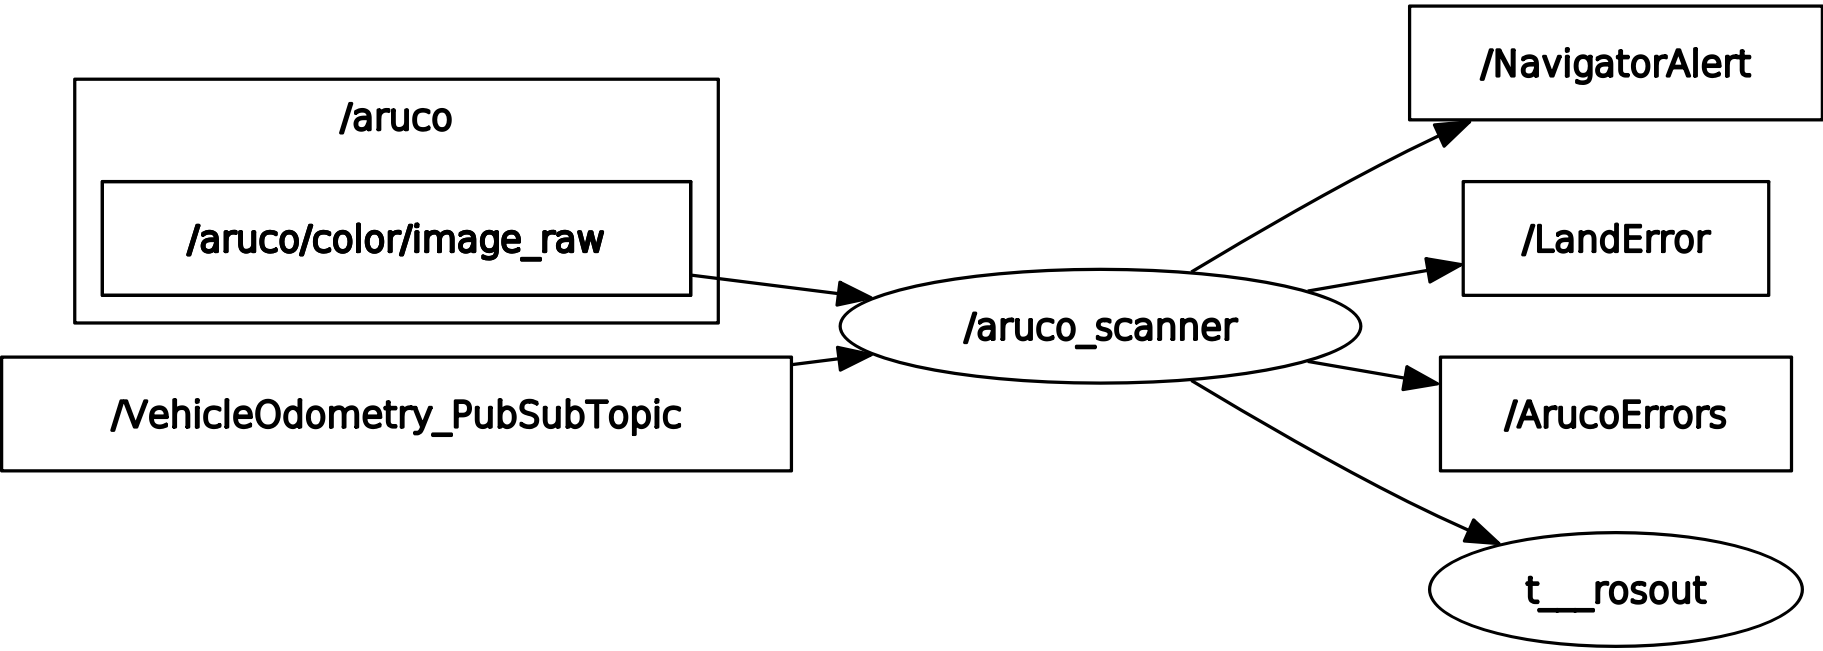
\includegraphics[width=0.7\textwidth]{figs/chapter3/ascan.png}
    \caption{Organizzazione del nodo \emph{aruco\_scanner}.}
    \label{fig:ascan}
\end{figure}

L'eseguibile comprende anche una modalità di calibrazione per poter determinare la distanza focale in pixel della camera in uso.\\
Durante la navigazione, il calcolo dell'errore di posizionamento rispetto al centro della piazzola viene effettuato in metri. Il modello matematico applicato per determinare ciascuna componente del vettore errore, estremamente semplice e basato sostanzialmente su similitudini tra triangoli, è noto come \emph{pinhole camera model} e può essere formulato come segue:
\begin{equation}
    W = \frac{P \cdot D}{F}
\end{equation}
dove $P$ è la lunghezza misurata in pixel dall'immagine, $D$ è la distanza dal landmark misurata usando l'altitudine del drone e compensando una eventuale elevazione della piazzola, $F$ è la distanza focale della camera in pixel e $W$ è la lunghezza effettiva in metri. Chiaramente questo approccio non è esente da errore: è stato rilevato che le misure sono attendibili fino al centimetro, una precisione sufficiente ma che richiede di troncare il risultato oppure azzerarlo quando troppo basso per escludere il rumore, ed inoltre essendo la camera inferiore solidale al drone queste misure hanno senso solo quando esso è livellato, problema a cui come si vedrà si è fatto fronte all'atto dell'acquisizione dei campioni negli altri moduli.
\clearpage

\begin{lstlisting}[language=C++, caption={Definizione del nodo \emph{aruco\_scanner}.}, label={lst:ascan}]
class ArucoScanner : public rclcpp::Node
{
public:
    ArucoScanner(bool calibrate,
                 float calib_hgt,
                 float focal_len,
                 std::vector<int> ids_good);

private:
    rclcpp::Publisher<ArucoDataVector>::SharedPtr error_vector_pub_;
    rclcpp::Publisher<Float32>::SharedPtr focal_len_pub_;
    rclcpp::Publisher<Bool>::SharedPtr stop_pub_;

    rclcpp::Subscription<VehicleOdometry>::SharedPtr odometry_sub_;
    rclcpp::Subscription<Image>::SharedPtr down_camera_sub_;

    rclcpp::CallbackGroup::SharedPtr camera_clbk_group_;
    rclcpp::CallbackGroup::SharedPtr odometry_clbk_group_;

    bool calibrating_;
    float calibration_hgt_;
    float focal_len_;
    std::atomic<float> drone_z_;
    std::vector<int> ids_good_;
    int pics_count_;

    cv::Ptr<cv::aruco::Dictionary> aruco_dictionary_;
    cv_bridge::CvImagePtr cv_ptr_;
    cv::Mat image_copy_;
    std::vector<int> ids_;
    std::vector<std::vector<cv::Point2f>> corners_;

    void odometry_msg_clbk(const VehicleOdometry::SharedPtr msg);
    void down_camera_clbk(const Image::SharedPtr msg);
};
\end{lstlisting}
\clearpage

\newsubsection{Navigator}
\indent Salendo ora al livello più alto nella gerarchia dei moduli, in Figura \ref{fig:navnode} è rappresentata la struttura del nodo incaricato di gestire la navigazione: il Navigator. Supponendo che i sistemi di localizzazione e controllo volo funzionino correttamente, le operazioni che deve realizzare sono:
\begin{itemize}
    \item decollo da una qualunque piazzola;
    \item esplorazione dell'ambiente alla ricerca del robot sconosciuto;
    \item navigazione da un qualunque punto della mappa verso una specifica piazzola;
    \item loop di ricerca attorno alla presunta posizione di una piazzola.
\end{itemize}
La sua struttura è illustrata nel Listing \ref{lst:navnode}. L'organizzazione è semplice, poiché si appoggia totalmente ai servizi offerti dagli altri package, offrendo un ulteriore livello di astrazione operativa alla logica di supervisione da cui è comandato tramite il servizio \emph{/Navigation}. L'odometria viene campionata dal topic \emph{/VehicleOdometry}, per fissare l'esatta posizione da cui decollare al fine di evitare drift in salita e per salvare la posizione della piazzola verso cui si sta andando durante la navigazione, se questa dovesse essere rilevata nel tragitto, anche grazie agli errori di posizionamento ricevuti dal topic \emph{/ArucoErrors}. Durante l'esplorazione è l'Aruco Scanner ad allertare il Navigator che un robot sconosciuto è stato individuato, tramite il topic \emph{/NavigatorAlerts}; in tal caso, il drone viene messo in hovering e viene formulata una richiesta al servizio della GCS per richiedere la sequenza di atterraggi all'operatore. Le operazioni di volo sono realizzate mediante i servizi \emph{/FlightControl} e \emph{/SetpointSetter} offerti dal Flight Control. I percorsi da seguire in ogni fase sono definiti per punti, ed ogni leg tra due punti intermedi viene ulteriormente discretizzata nella routine \emph{reach\_point}, la quale richiede poi di attendere il raggiungimento di ogni punto mediante l'apposito servizio del Flight Control. Per velocizzare l'andatura, il raggio di confidenza in cui si suppone che un setpoint sia stato raggiunto viene allargato e ristretto dinamicamente secondo necessità. I percorsi d'esplorazione sono predefiniti per ogni piazzola in base alla mappa, al fine di massimizzare la probabilità di trovare il robot sconosciuto, mentre quelli di navigazione vengono richiesti ad un altro nodo che si occupa di calcolarli.

\begin{figure}
    \centering
    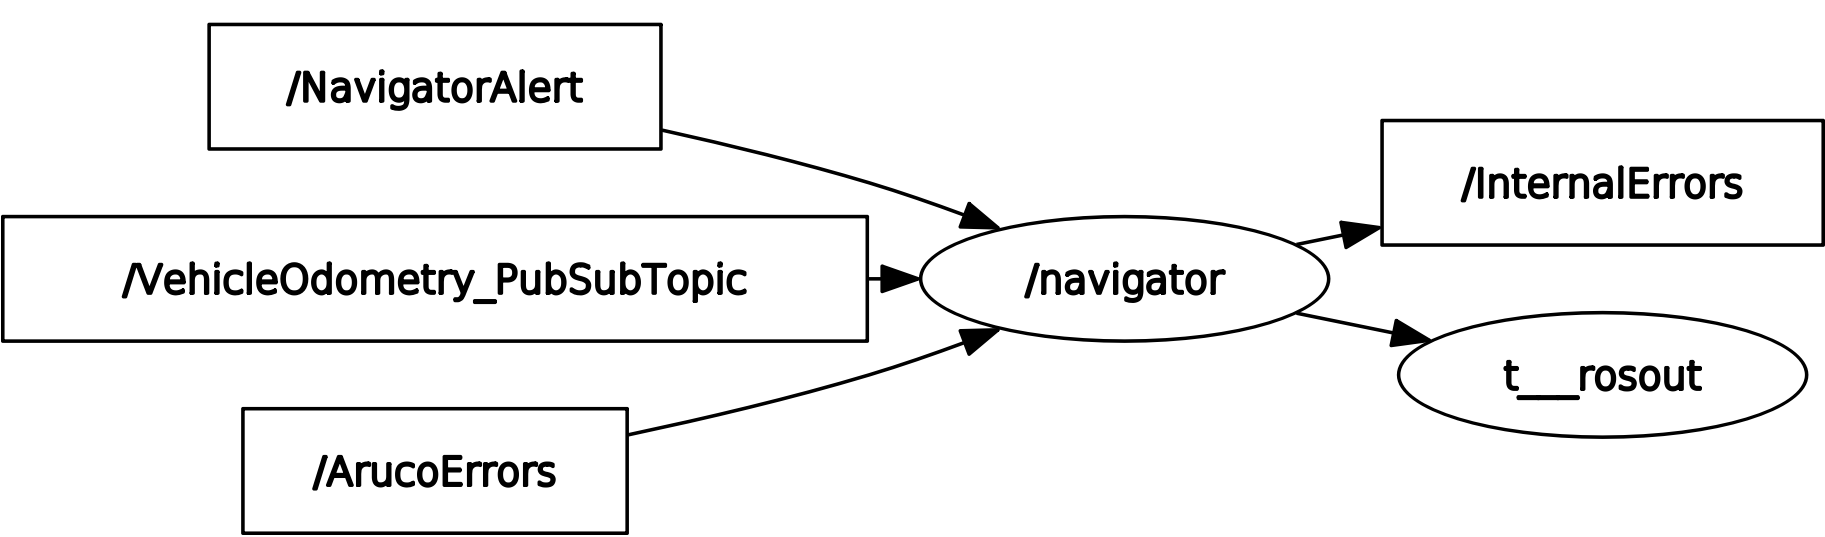
\includegraphics[width=0.7\textwidth]{figs/chapter3/navigator.png}
    \caption{Organizzazione del nodo \emph{navigator}.}
    \label{fig:navnode}
\end{figure}

\begin{lstlisting}[language=C++, caption={Definizione del nodo \emph{navigator}.}, label={lst:navnode}]
class Navigator : public rclcpp::Node
{
public:
    Navigator();

private:
    rclcpp::Subscription<VehicleOdometry>::SharedPtr odometry_sub_;
    rclcpp::Subscription<Bool>::SharedPtr alert_sub_;
    rclcpp::Subscription<ArucoDataVector>::SharedPtr pad_sub_;

    rclcpp::Service<Navigation>::SharedPtr navigation_srv_;

    rclcpp::CallbackGroup::SharedPtr odometry_clbk_group_;
    rclcpp::CallbackGroup::SharedPtr alert_clbk_group_;
    rclcpp::CallbackGroup::SharedPtr navigation_clbk_group_;

    rclcpp::Client<FlightControl>::SharedPtr flight_control_client_;
    rclcpp::Client<LandingSequence>::SharedPtr landing_sequence_client_;
    rclcpp::Client<PathFinder>::SharedPtr path_finder_client_;
    rclcpp::Client<SetpointSetter>::SharedPtr setp_client_;
    rclcpp::Client<ArucoScanner>::SharedPtr scanner_client_;

    rclcpp::Publisher<InternalError>::SharedPtr error_pub_;

    std::mutex odom_lock_;
    float drone_x_, drone_y_, drone_z_;

    std::atomic<bool> stop_;

    std::atomic<int> curr_pad_;
    float last_pad_pos_[2];

    void odometry_clbk(const VehicleOdometry::SharedPtr msg);
    void alert_clbk(const Bool::SharedPtr msg);
    void pad_clbk(const ArucoDataVector::SharedPtr msg);
    void navigation_clbk(const Navigation::Request::SharedPtr request,
                         const Navigation::Response::SharedPtr response);

    void takeoff(const Navigation::Request::SharedPtr req,
                 const Navigation::Response::SharedPtr resp);
    void explore(const Navigation::Request::SharedPtr req,
                 const Navigation::Response::SharedPtr resp);
    void navigate(const Navigation::Request::SharedPtr req,
                  const Navigation::Response::SharedPtr resp);
    void search_pad(const Navigation::Request::SharedPtr req,
                    const Navigation::Response::SharedPtr resp);

    bool reach_point(float target_x, float target_y, float target_z,
                     bool exploring, bool check_yaw, bool force_disc, float step,
                     const Navigation::Response::SharedPtr resp);
};
\end{lstlisting}

\newsubsection{Path Finder}
\indent Non appena un robot sconosciuto è stato rilevato e l'operatore alla GCS ha trasmesso la sequenza di atterraggi da compiere, nonché dopo ogni decollo relativo a tale sequenza, si rende necessario navigare dal punto in cui ci si trova fino alla posizione della piazzola successiva. Il calcolo del percorso migliore dalla posizione corrente a quella desiderata è effettuato dal nodo \emph{Path Finder}, la cui struttura è illustrata nel Listing \ref{lst:pathfnode}. Tale nodo offre semplicemente il servizio \emph{/PathFinder} al Navigator, tramite il quale viene richiesto e restituito il percorso ottimo punto per punto, nel caso esista. L'algoritmo impiegato per il calcolo è A*, applicato su un grafo ricostruito dal pointcloud di una mappa accurata del campo acquisita mediante lo stesso sistema di localizzazione del drone, ossia ORB\_SLAM2. Oggetto di questo lavoro è stata la realizzazione e integrazione di un nodo ROS 2 che offrisse tale servizio, mentre l'implementazione dell'algoritmo si deve al collega Alessandro Tenaglia, con un sentito ringraziamento personale. L'algoritmo tiene inoltre conto delle dimensioni del drone, con dei margini di sicurezza, assicurandosi di poterlo effettivamente spostare nei punti che trova. Un esempio d'esecuzione è mostrato in Figura \ref{fig:pathfpath}, che evidenzia gli ostacoli e i punti del percorso.

\begin{figure}
    \centering
    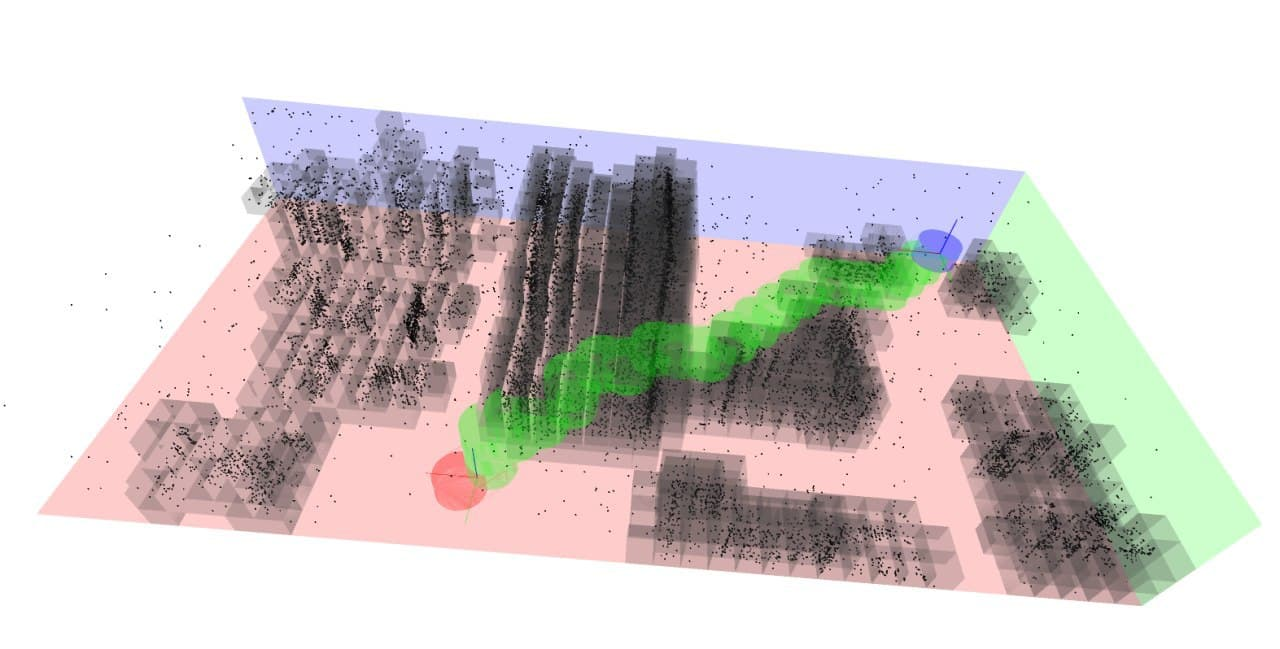
\includegraphics[width=\textwidth]{figs/chapter3/pathfpath.jpg}
    \caption{Risultato dell'algoritmo A* per il calcolo del percorso da piazzola 6 a 3.}
    \label{fig:pathfpath}
\end{figure}

\vspace{0.5cm}
\begin{lstlisting}[language=C++, caption={Definizione del nodo \emph{path\_finder}.}, label={lst:pathfnode}]
class PathFinderNode : public rclcpp::Node
{
public:
    PathFinderNode(char *config_file, char *space_file);

private:
    float xStart, yStart, zStart, xMargin, yMargin, zMargin, yaw;
    CubeSpace *space;
    rclcpp::Service<PathFinder>::SharedPtr path_finder_srv_;
    void path_finder_clbk(PathFinder::Request::SharedPtr request,
                          PathFinder::Response::SharedPtr response);
};
\end{lstlisting}

\newsubsection{Ground Control Station}
\indent In esecuzione sul PC adibito a Ground Control Station è stato posto un nodo, denominato appunto \emph{GCS}, che consentisse all'operatore di inserire la sequenza degli atterraggi da eseguire dopo aver individuato il robot sconosciuto. La struttura di questo nodo è illustrata nel Listing \ref{lst:gcs} ed è estremamente semplice, in quanto si riduce ad un server per il servizio \emph{/LandingSequence} la cui callback offre all'operatore un'interfaccia a riga di comando per inserire la sequenza. È stata anche tentata la trasmissione, mediante un opportuno topic, delle foto dei robot sconosciuti tramite questo nodo, ma la procedura è stata rimossa in quanto come si è puntualizzato nel capitolo precedente la trasmissione di messaggi di grandi dimensioni come le immagini è al momento problematica per i DDS su reti soggette a perdita, come WiFi. Pertanto, tale funzionalità è stata rimpiazzata da uno script di shell che trasferisce via \emph{scp} tutte le nuove foto scattate.
\vspace{1cm}
\begin{lstlisting}[language=C++, caption={Definizione del nodo \emph{gcs}.}, label={lst:gcs}]
class GCSNode : public rclcpp::Node
{
public:
    GCSNode();

private:
    rclcpp::Service<LandingSequence>::SharedPtr landing_seq_srv_;
    rclcpp::CallbackGroup::SharedPtr land_seq_clbk_group_;

    void landing_seq_callback(const LandingSequence::Request::SharedPtr request,
                              const LandingSequence::Response::SharedPtr response);
};
\end{lstlisting}

\newsubsection{Precision Landing}
\indent Una volta raggiunta la presunta posizione di una piazzola, ed accertato tramite la camera inferiore e l'Aruco Scanner che essa è in vista, ci si deve atterrare. Questa operazione è a carico di un nodo, denominato \emph{precision\_lander} e facente parte del package \emph{Precision Landing}, la cui struttura è mostrata nel Listing \ref{lst:pland} e in Figura \ref{fig:pland}.

\begin{figure}
    \centering
    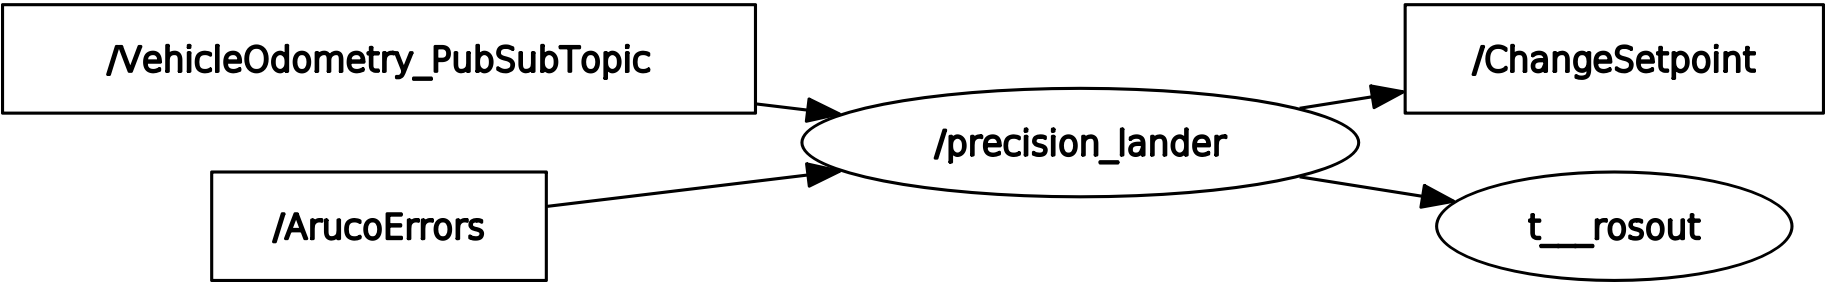
\includegraphics[width=0.7\textwidth]{figs/chapter3/pland.png}
    \caption{Struttura del nodo \emph{precision\_lander}.}
    \label{fig:pland}
\end{figure}
\vspace{0.5cm}
\begin{lstlisting}[language=C++, caption={Definizione del nodo \emph{precision\_lander}.}, label={lst:pland}]
class PrecisionLander : public rclcpp::Node
{
public:
    PrecisionLander();

private:
    rclcpp::Publisher<afg_interfaces::msg::ChangeSetpoint>::SharedPtr vel_setp_pub_;
    rclcpp::Client<FlightControl>::SharedPtr flight_control_client_;
    rclcpp::Client<SetpointSetter>::SharedPtr setp_set_client_;

    rclcpp::Subscription<ArucoDataVector>::SharedPtr aruco_data_sub_;
    rclcpp::Subscription<VehicleOdometry>::SharedPtr vehicle_odometry_sub_;
    rclcpp::Service<PrecLanding>::SharedPtr prec_landing_srv_;

    rclcpp::CallbackGroup::SharedPtr aruco_data_clbk_group_;
    rclcpp::CallbackGroup::SharedPtr odometry_clbk_group_;
    rclcpp::CallbackGroup::SharedPtr prec_landing_clbk_group_;

    double drone_x_, drone_y_, drone_z_;
    double drone_vx_, drone_vy_, drone_vz_;
    double drone_roll_, drone_pitch_, drone_yaw_;
    std::mutex odometry_status_lock_;

    std::atomic<int> landing_id_;

    bool do_prec_landing_;
    std::mutex prec_landing_lock_;
    std::condition_variable prec_landing_cv_;

    std::atomic<bool> timeo_expired_;
    clock_t start_;
    clock_t t_now_, t_prec_;
    double t_passed_;

    float x_err_int_, y_err_int_;
    float x_err_der_, y_err_der_;
    float x_err_old_, y_err_old_;
    float z_ref_, z_init_;
    float land_alt_;
    float land_yaw_;
    float last_x_, last_y_;

    bool is_on_target(float x_err, float y_err);

    void aruco_data_clbk(const ArucoDataVector::SharedPtr msg);
    void odometry_states_clbk(const VehicleOdometry::SharedPtr msg);
    void precision_landing_clbk(const PrecLanding::Request::SharedPtr request,
                                const PrecLanding::Response::SharedPtr response);
};
\end{lstlisting}
Come si evince dal listato, questo nodo è programmato in modo concorrente: vi è una callback che campiona l'odometria per capire come è posizionato ed orientato il drone totalmente in parallelo rispetto al resto, una callback dal servizio \emph{/PrecisionLanding} tramite cui può essere richiesta la procedura e una dal topic \emph{/ArucoErrors} da cui viene estratto l'errore di posizionamento rispetto alla piazzola. Quando giunge una richiesta per il servizio, il thread che la gestisce attiva il processamento dei dati nella callback da \emph{/ArucoErrors}, dove è implementato l'algoritmo di controllo. Tutte le operazioni di volo sono ancora una volta gestite mediante i servizi ed i topic offerti da Flight Control, ed il termine della procedura è soggetto a timeout e gestito mediante opportuni meccanismi di segnalazione tra thread basati su condition variables. Se tutto procede senza intoppi, la callback da \emph{/ArucoErrors} corregge progressivamente l'allineamento del drone facendolo scendere ed infine segnala all'altro thread, rimasto in attesa, che questo è pronto per la discesa finale. Sarà la callback del servizio, una volta riattivata, a richiedere l'esecuzione dell'atterraggio a Flight Control.\\
L'algoritmo di controllo per correggere l'allineamento ed eseguire la discesa preliminare è stato sviluppato a più riprese: inizialmente si è testata in simulazione, con buoni risultati, una terna di PID\footnote{Il PID è una tipologia standard di controllori che si basano sulla composizione di un'azione di controllo finalizzata ad azzerare un segnale d'errore, e calcolata sulla base di esso, la sua derivata rispetto al tempo e la sua somma integrale entro un opportuno intervallo.} sui vari assi che controllasse il drone in velocità lineare inviando messaggi sul topic \emph{/ChangeSetpoint}. Tale soluzione si è rivelata però, a pochi giorni dalla competizione, inapplicabile per problemi di carico del sistema che inficiavano le prestazioni della camera: il rate di campionamento era infatti troppo basso e troppo variabile per consentire l'implementazione di un qualunque algoritmo di controllo veloce. Per queste ragioni e per il pochissimo tempo a disposizione è stato implementato un algoritmo più semplice denominato \emph{Land Corrector}: l'errore di posizionamento campionato dall'Aruco Scanner col drone livellato viene usato per calcolare un nuovo setpoint di posizione, che si raggiunge con stabilizzazione formulando una richiesta al servizio \emph{/SetpointSetter}; tale procedura viene ripetuta, diminuendo la quota se il drone è sufficientemente allineato e stabile, fino al raggiungimento di un'altitudine limite al di sotto della quale viene iniziata la discesa finale.

\newsection{Realizzazione}
console, checklist, affidabilità, atterraggi, risultato
\indent
